\documentclass[11pt,a4paper,twoside]{article}
\usepackage[T1]{fontenc}
\usepackage[utf8]{inputenc}

\usepackage{lipsum}
\usepackage{authblk}
\usepackage[top=3cm, bottom=3cm, left=3cm, right=3cm]{geometry}
\usepackage{fancyhdr}
%
\usepackage{adjustbox}
\usepackage{caption}
\usepackage{subcaption}
\usepackage{tabularx}
%\usepackage{enumitem}
\usepackage{algorithm}
\usepackage{graphicx,epsfig} 
\usepackage[noend]{algpseudocode}
\usepackage{algpseudocode}
\usepackage{amsmath, amsfonts,amssymb,stmaryrd,moreverb,multirow}
\usepackage{enumitem}
\usepackage[sort&compress]{natbib}
\usepackage[colorlinks,bookmarksopen,bookmarksnumbered,citecolor=red,urlcolor=red]{hyperref}
%
%\renewcommand{\baselinestretch}{1.5}
%%% Modify autoref function
\newcommand{\Aref}[1]{%
	\begingroup%
	\def\chapterautorefname~##1\null{Ch.~##1\null}%
	\def\sectionautorefname~##1\null{Section~##1\null}%
	\def\subsectionautorefname~##1\null{Section~##1\null}%
	\def\figureautorefname~##1\null{Fig.~##1\null}%
	\def\tableautorefname~##1\null{Table~##1\null}%
	\def\equationautorefname~##1\null{Eq.~##1\null}%
	\autoref{#1}%
	\endgroup%
}
%%
\newcommand{\aref}[1]{%
	\begingroup%
	\def\chapterautorefname~##1\null{Chapter~##1\null}%
	\def\sectionautorefname~##1\null{Section~##1\null}%
	\def\subsectionautorefname~##1\null{Section~##1\null}%
	\def\subsubsectionautorefname~##1\null{Section~##1\null}%
	\def\figureautorefname~##1\null{Fig.~##1\null}%
	\def\tableautorefname~##1\null{Table~##1\null}%
	\def\equationautorefname~##1\null{Eq.(##1)\null}%
	\def\algorithmautorefname~##1\null{Alg.(##1)\null}%
	\autoref{#1}%
	\endgroup%
}
% ADD THE FOLLOWING COUPLE LINES INTO YOUR PREAMBLE
\let\OLDthebibliography\thebibliography
\renewcommand\thebibliography[1]{
	\OLDthebibliography{#1}
	\setlength{\parskip}{0pt}
	\setlength{\itemsep}{0pt plus 0.3ex}
}


%%%%% end %%%%%%%%%
\graphicspath{ {./figures/} }

%%%

\renewenvironment{abstract}{%
	%\hfill
	\begin{center}
		\begin{adjustbox}{minipage=0.90\textwidth,center} 
			\rule{\textwidth}{0.5pt}}
		{\par\noindent\rule{\textwidth}{0.5pt}  
		\end{adjustbox}
	\end{center} 
}

\makeatletter

\renewcommand\@maketitle{%
	%\hfill
	\begin{adjustbox}{minipage=0.90\textwidth,center}
		\begin{center}
			\vskip 2em
			\let\footnote\thanks 
			{\LARGE \@title \par }
			\vskip 1.5em
			{\large \@author \par}
		\end{center}
	\end{adjustbox}
	\vskip 2em \par
}
\makeatother
%\pagestyle{fancy}
\begin{document}
	\title{An Adaptive Fully Discontinuous Galerkin Level Set Method for Incompressible Multiphase Flows}
	\author[1]{A. Karakus}
	\author[2]{T. Warburton}
	\author[1]{M.H. Aksel}
	\author[1]{C. Sert}
	%%%%
	\affil[1]{\small{\textit{Department of Mechanical Engineering, Middle East Technical University\\ Ankara, 06800 Turkey.}}}
	\affil[2]{\textit{\small{Department of Mathematics, Virginia Tech, Blacksburg, VA 24061-0123}}}
	
	\renewcommand\Authands{ and }
	\date{\vspace{-5ex}}
	
	\maketitle
	
	\begin{abstract}
		This study focuses on the development of a high-order discontinuous Galerkin method for the solution of unsteady, incompressible, multiphase flows with level set interface formulation.  Nodal discontinuous Galerkin discretization is used for incompressible Navier-Stokes, level set advection and reinitialization equations on adaptive unstructured elements. Implicit systems arising from the semi-explicit time discretization of  the flow equations are solved with a $ p $-multigrid preconditioned conjugate gradient method which minimizes the memory requirements and increase overall run time performance. Computations are localized mostly near the interface location in the adaptive method to reduce computational cost without sacrificing the accuracy. Efficiency, local high-order accuracy and mass conservation of the method are confirmed through distinct numerical test cases of sloshing, dam break and Rayleigh-Taylor instability. \\
		\textbf{Keywords:}  High-order, Discontinuous Galerkin, Incompressible Multiphase Flows,  Level Set, Adaptivity, Multigrid
	\end{abstract}

	
	\textcolor{red}{\textcolor{red}{TODO}}: Yazılmış, ama artık kullanılmayan şeyleri bir temizlemek gerek. Cok fazla oyle yer var.

	\section{Introduction}
	%%
	Multiphase flows occur in many areas of practical importance such as flow-structure interaction, air-water interfacial dynamics, phase change problems, reacting flows etc. Numerical prediction of the deformable interfaces in these complex flows are challenging due to discontinuity in the material properties, varying topology and wide range of scales.
		
	%%
	Numerous numerical methods were proposed to represent the phase dynamics in incompressible flows. These methods can be classified as interface tracking and interface capturing. The former group are Lagrangian or semi-Lagrangian, where the mesh or massless particles explicitly represents the interface \cite{unverdi_front-tracking_1992,harlow_numerical_1965}. Interface tracking approaches are generally accurate and robust but difficult to use when the interface encounters topological changes. Interface capturing methods, Volume of Fluid (VOF) \cite{hirt_volume_1981} and level set (LS) \cite{osher_fronts_1988},  are Eulerian  i.e. an implicit function defined on a fixed grid represents the interface. Specifically, VOF methods are widely used in multiphase flow simulations due to their natural  conservation properties and efficiency, but reconstruction of the interface from volume fraction data and obtaining geometry dependent properties, such as interface  normal and curvature, are difficult to compute. 
		
	%%
	LS method addresses the  problems of interface tracking and VOF methods. In the LS method, an interface between the phases is represented by a specified contour level of a continuous function. This implicit interface representation offers many advantages such as straightforward extension from 2D to 3D, simple handling of topological changes and easy calculation of geometric properties. The main difficulty with use of the LS method is the need to control mass loss present in the method. Various techniques have been proposed to improve the conservation properties of the original method. Popular ones are combining LS with VOF \cite{sussman_coupled_2000} or with a semi-Lagrangian particle method \cite{enright_hybrid_2002} and applying additional mass correction procedures \cite{sussman_efficient_1999,wang_hybrid_2012}. Common to all these approaches is the fact that simplicity and computational efficiency of the original LS method is partly lost.  In fact, mass loss problem of the LS method is more inherent in the discretization scheme used than the formulation itself \cite{marchandise_quadrature-free_2006,karakus_gpu-accelerated_2016}.
		
	%%
	The discontinuous Galerkin (DG) methods (\cite{hesthaven_nodal_2008} and references therein)  are a class of finite element methods that make use of completely discontinuous spatial discretization. The DG methods have excellent dissipation properties achieved by local high-order polynomial approximations to overcome  the mass loss problem of the LS formulation. For this reason, using DG for LS advection gives more accurate results compared with the widely used essentially non-oscillatory (ENO) type schemes \cite{sussman_discontinuous_2003,karakus_gpu-accelerated_2016}. DG level set modeling is also applied in incompressible multiphase flow simulations i.e. it is combined with  a stabilized finite element \cite{marchandise_stabilized_2006,marchandise_stabilized_2007} and a conservative finite difference \cite{owkes_discontinuous_2013} flow solvers. These hybrid methods require interpolation of the velocity field obtained from the lower-order flow solver to higher-order discontinuous polynomial space in each time step. Fine grids are needed for flow solver which may became computationally inefficient when high-order interpolation orders are used for LS evolution.  
	
	%%
	Multiphase flows are generally highly dynamic in the sense that location and topology of the interface change considerably during the simulation. In a fixed grid approach, resolution should be increased in whole domain to  capture the full physics of interface,  which obviously creates unnecessary burden in computational time. Adaptive mesh refinement (AMR) techniques decrease the computational effort by increasing the resolution in the vicinity of  interface with keeping coarse grid at less dynamic regions.  There are some adaptive LS methods for multiphase flows based on the low-order finite difference/volume schemes on structured Cartesian grid and tree type data structures \cite{sussman_adaptive_1999,sussman_parallelized_2005,losasso_spatially_2006}. Unstructured anisotropic mesh refinement is also coupled with the low-order finite element flow solution with higher-order  DG interface modeling \cite{marchandise_stabilized_2006}. This type refinement strategies are based on the conformal discretization that each face can only be shared by two elements. AMR algorithm should handle the complicated interpolation between grids and mesh transition to ensure the conformity \cite{kopera_analysis_2014}. Global re-meshing or iteratively optimized local modifications may become inefficient when frequent adaptation is needed as in the multiphase flow simulations. Due to relaxed strong elemental connectivity, DG methods can be easily  used on unstructured elements with hanging nodes \cite{eskilsson_hp-adaptive_2011,kopera_analysis_2014} that enables the fast adaptation with accurate interpolation between the grids.          
	
	%%
	In this study, we present  a high-order, fully discontinuous Galerkin method for immiscible, incompressible multiphase flows on adaptive unstructured grids. The proposed method allows to capture interface topology accurately  in simulating wide range of flow regimes with high density/viscosity ratios and offers good mass conservation even in relatively coarse grids while keeping the simplicity of the level set interface modeling. Outline of this paper is as follows: the governing equations of the problem and notation used in the numerical scheme are described in  \aref{Sec.Numerical Method}. Then, time and high-order discontinuous Galerkin spatial discretizations and matrix-free solution techniques are presented. At the end of the section, local interface model with reinitialization of the level set function and adaptive mesh refinement strategy  are described.   Finally, \aref{Sec.Numerical_Tests} gives  distinct numerical test cases to show the accuracy and mass conservation of the method. 	
	%%
	%=============================================================================%
	\section{Governing Equations}
	\label{Sec.Governing Equations}
	
	%%
	Incompressible, laminar flow of two immiscible, non-reacting fluids are  governed by the Navier-Stokes equations defined on the domain $\Omega = \Omega_1\cup\Omega_2$. Here, subscripts $ 1 $ and $ 2 $ denote the sub-domains of the first and second fluids, respectively. Domain boundary is represented by $ \partial \Omega $ while the $ \Gamma = \Omega_1\cap\Omega_2$ denotes the interface separating the fluid phases. Problem domain, $\Omega$ is fixed  but two fluid domains, $ \Omega_1$ and $\Omega_2 $  and the interface, $ \Gamma $ change in time.  
	
	The  non-dimensional, incompressible Navier-Stokes and the continuity equations  on  $ \Omega $ can be written as,
	%   
	\begin{equation}
	\label{Eq.NonDimensionalNavierStokes}
	\begin{aligned}
	\frac{\partial \mathbf{u}}{\partial t} + \left(\mathbf{u}\cdot\nabla\right)\mathbf{u} = -\frac{\nabla p}{\rho}+ \frac{1}{ \text{Re}\rho} \nabla\cdot\left(2\mu S \right) +\frac{\mathbf{e}_g}{\text{Fr}^2} + \frac{\kappa \mathbf{n}_\Gamma}{\text{We}},  \quad  \nabla\cdot\mathbf{u} = 0,   \quad   \forall \mathbf{x} \in \Omega 
	\end{aligned}
	\end{equation}
	%
	where $ \textbf{u} $ denotes the velocity field,  $ p $ is the static pressure, $ \rho$  is the density, $ \mu$ is the dynamic viscosity, $ S = \frac{1}{2}\left( \nabla \mathbf{u} + \nabla \mathbf{u}^T\right) $ is the deformation rate tensor, $ \mathbf{e}_g $ is the direction of the gravitational acceleration, $ \mathbf{n}_\Gamma $ is the unit normal of $ \Gamma $  and $ \kappa = \nabla\cdot\mathbf{n}_{\Gamma} $ is the local curvature of the interface. The non-dimensional Reynolds, Froude and Weber numbers  are defined using the reference variables denoted with subscript $ R $ as  $ \text{Re} = \rho_R U_R L_R / \mu_R $, $ \text{Fr} = U_R/ \sqrt{ gL_R}  $  and $ \text{We} =  \rho_R U_R L_R/ \sigma_R$, respectively (\textcolor{red}{TODO}: Bu referans degerler problemler cozulurken verilecek mi?). Hereafter, $ \mathbf{F} = \frac{\mathbf{e}_g}{\text{Fr}^2} $ is used as the non-dimensional body force term. In this study, surface tension forces are neglected but the method still governs many practical, large scale problems where curvature is too small to contribute to the governing equations.
		
	%%
	Level set method is used to model phase dynamics where the interface is represented by at least a Lipschitz continuous function, $ \phi  $ which is positive in one fluid domain and negative in the other. The zero contour of the implicit LS function, i.e. $ \phi(\textbf{x}, t) = 0 $ defines the current location of the interface. Using this definition, $ \rho $ and $ \mu $ can be globally defined as,  
	%
	\begin{equation}
	\label{Eq.GlobalDensityViscosity}
	\begin{aligned}
	\rho(\phi) = \rho_1 H(\phi) + \rho_2\left( 1-H(\phi) \right) \\
	\mu(\phi) = \mu_1 H(\phi) + \mu_2\left( 1-H(\phi) \right)
	\end{aligned}
	\end{equation}
	where $ H(\phi) $ is the Heaviside step function. Time evolution of the interface can be obtained by simple advection of the level set function with the known velocity field, as given below
	%
	\begin{equation}
	\label{Eq.LevelSet_1}
	\frac{\partial \phi}{\partial t}+\mathbf{u} \cdotp \nabla \phi =  0
	\end{equation}
	%
	
    %%	
	In the interface model, LS is kept as signed distance function such that $ \lvert \nabla \phi \rvert  = 1$ is fulfilled. Evolution of the interface destroys the regularity of the LS function and creates very large or small gradients near the interface. Reinitialization is required to replace the distorted LS with more desired signed distance function to enhance the accuracy of interface representation and  given in \Aref{Sec.Interface Modeling}. 

%	In this study, reinitialization is not used at the end of each time step, unlike the low-order level set methods \cite{sussman_level_1994,nagrath_computation_2005,smolianski_finite_2005}, which reduces the computational cost. (\textcolor{red}{TODO}: Peki ne yapıldı bunun yerine?)
	
		
	
	\section{Numerical Method}
	\label{Sec.Numerical Method}
	
	%%
	%=============================================================================%
	\subsection{Preliminaries and Notations}
	
	%%%
	We assume that $ d $ dimensional domain $\Omega\subset R^{d}$ is well approximated by the computational domain, $\Omega_{h}$ having boundaries $ \partial \Omega_{h} $, which can be Dirichlet, $  \partial \Omega_{D}$ or Neumann type, $  \partial \Omega_{N}$. $ \Omega_{h}$ is partitioned into non-overlapping, possibly nonconforming triangular/tetrahedral elements, $\Omega_{h} = \cup_{k=1}^{K} D_k$. Two element domains, $D_{k}^{-}$ and $D_{k}^{+}$ of the triangulation $\Omega_{h}$ has a common face if $\partial D_{k}^{-} \cap \partial D_{k}^{+} \neq \emptyset$, where $ \partial D_{k} $ denotes the element interface. $\textbf{n}^{-}=-\textbf{n}^{+}$ be the unit outward normal vector of $\partial D_{k}$. $ \varphi_k^{-}$ and $\varphi_k^{+}$ denote the traces of a scalar function, $\varphi$ when evaluated at $\partial D_{k}^{-}$ and  $\partial D_{k}^{+}$, respectively. According to this definition average and jump operators for a scalar valued function can be  defined as,
	%
	\begin{equation}
	\label{Eq.AverageJumpScalar}
	\begin{aligned}
	\{\varphi \}        &= \frac{\varphi^{-} + \varphi^{+}}{2},   &                 \llbracket \varphi  \rrbracket  & = \varphi^{-} -\varphi^{+}         
	\end{aligned}
	\end{equation}
	When $ \varphi $ is a vector-valued function, the above operators act on it component wise. On  Dirichlet or Neumann boundaries, normal vectors point outward to $ \Omega_h $, and average and jump operators are equal to the trace of function $ \varphi $ unless otherwise stated.  
	
	%%%
	The discontinuous approximate spaces are $  \mathcal{V}_N  = \{ v\in L^2(\Omega)\lvert v \lvert_{D_{k}} \in \mathcal{P}_N(D_{k}), \; \forall D_{k} \in \Omega_h \} $
	and its vector version, $ \mathcal{V}_N^d $. $\mathcal{P}_N(D_{k}) $ is the space of discontinuous piecewise polynomial functions of degree $N\geq 1$ on each elemental domain. Lagrange polynomials are constructed as the basis for this polynomial space using Warp$\&$Blend nodes \cite{warburton_explicit_2006} and orthonormal Proriol-Koornwinder-Dubiner (PKD) \cite{Proriol_1957,koornwinder_1975,dubiner_spectral_1991} polynomials. Let $ (\cdot , \cdot)_{D_{k}} $ represent the inner product computed over the volume of the element $ k $. Similarly, let $ (\cdot , \cdot)_{\partial D_{k}}$ denote the inner product taken along the element boundaries. 
		
	
	%%=============================================================================%
	\subsection{Temporal Discretization}
	
	%%
	A high-order splitting scheme \cite{karniadakis_high-order_1991} is used for the temporal discretization of the flow equations. The scheme is semi-implicit, in which non-linear terms are integrated explicitly and linear terms are treated implicitly. Second order backward differentiation is used for the unsteady term and second order extrapolation is used for the non-linear terms. With this implementation, \aref{Eq.NonDimensionalNavierStokes} can be advanced from time levels, $ n $ to $n+1 $ by solving the following semi-discrete equations decomposed into three fractional steps for $ \mathbf{u} $. 
	%%
	\begin{subequations}
		\label{Eq.TimeSplittingScheme}
		\begin{align}
		\frac{\hat{ \mathbf{u}}- \alpha_0 \mathbf{u}^{n} -\alpha_1 \mathbf{u}^{n-1}  } {\Delta t} &= \beta_0 \left( \left(\mathbf{u}^n \cdot\nabla\right)\mathbf{u}^n  +\mathbf{F}^n \right)  + \beta_1 \left( \left(\mathbf{u}^{n-1} \cdot\nabla\right)\mathbf{u}^{n-1}  + \mathbf{F}^{n-1} \right) \label{Eq.TimeSplittingScheme-1}\\
		\frac{ \hat{   \hat{ \mathbf{u}  }} - \hat{\mathbf{u}}} {\Delta t} &= -\frac{1}{\rho(\phi)}\nabla p^{n+1}  \label{Eq.TimeSplittingScheme-2}  \\
		\frac{ \gamma_0 \mathbf{u} ^{n+1}- \hat{\hat{\mathbf{u}}} } {\Delta t} &= \frac{1}{ \rho(\phi)Re}\nabla\cdot\mu(\phi)\nabla\mathbf{u}^{n+1} \label{Eq.TimeSplittingScheme-3}
		\end{align}
	\end{subequations}
	%%
	The coefficients, $ \alpha$, $ \beta $ and $ \gamma$ correspond to a second order stiffly stable scheme and their values can be found in \cite{karniadakis_high-order_1991,karniadakis_spectral/hp_2005}. In the splitting scheme, pressure is decoupled from the velocity, which avoids spurious pressure modes and enable to use equal order approximations for both flow fields.     
	
	
	
	%%%
	In the first step, nonlinear terms and body forces are advanced explicitly by a second order stiffly stable extrapolation scheme. Then, incompressibility constraint is enforced in \aref{Eq.TimeSplittingScheme-2} by forcing the second intermediate velocity field, $ \hat{ \hat{ \mathbf{u}  }} $ to be divergence free. Finally, a modified Helmholtz equation is solved for the viscous terms to obtain next time level velocities. In \cite{guermond_overview_2006}, it was demonstrated that the splitting scheme  preserves the optimal second order accuracy.  
	
	
	%%
	%=============================================================================%
	\subsection{Nonlinear Treatment}
	
	%%%
	The first step of the splitting scheme requires approximation of the nonlinear term, which is written in divergence form as  $ \left(\mathbf{u}\cdot\nabla\right)\mathbf{u}  = \mathbf{u}\cdot\nabla \mathbf{u} + \mathbf{u}\nabla\cdot\mathbf{u} = \nabla\cdot\left(   \mathbf{u}\otimes\mathbf{u}\right)$, where $ \mathbf{u}\otimes\mathbf{v} = u_i v_j , \;i,j = 1,\cdots,d $. Let $ \mathbf{u} $  is approximated by $ \mathbf{u}_h \in \mathcal{V}_N^d$. Multiplying the nonlinear term with a test function, $ \mathbf{v}_h \in \mathcal{V}_N^d $, integrating over element  domain and performing integration by parts, we obtain the following local statement.
	%
	\begin{equation}
	\label{Eq.NonlinearTermDiscretization_1}
	\begin{aligned}
	\left(\nabla\cdot\left(  \mathbf{u}_h\otimes\mathbf{u}_h\right),\mathbf{v}_h\right)_{D_{k}} =
	-\left(   \mathbf{u}_h\otimes\mathbf{u}_h, \nabla\cdot\mathbf{v}_h \right)_{D_{k}} 
	+\left(  \mathbf{n}\cdot   \llbracket \mathbf{u}_h \otimes\mathbf{u}_h\rrbracket, \mathbf{v}_h\right)_{\partial D_k}
	\end{aligned}
	\end{equation}
	
	
	%%%
	Due to the discontinuous approximation space, the flux function, $\mathbf{n}\cdot   \llbracket \mathbf{u}_h \otimes\mathbf{u}_h\rrbracket $, in the boundary contribution is not uniquely defined and hence replaced  with the local Lax-Friedrich numerical flux, $ \tilde{F}_c $
	\begin{equation}
	\label{Eq.NonlinearTermDiscretization_2}
	\begin{aligned}
	\tilde{F}_{C} = \mathbf{n} \cdot  \lbrace \mathbf{u}_h \otimes\mathbf{u}_h \rbrace  + \frac{1}{2}\Lambda_{\partial D_k} \llbracket  \mathbf{u}_h  \rrbracket 
	\end{aligned}
	\end{equation}
	%%%
	Here, $ \Lambda_{\partial D_k} = \max_u | \mathbf{n}\cdot\frac{\partial \left(\mathbf{u}_h \otimes\mathbf{u}_h\right) }{\partial \mathbf{u}_h}|$ is the maximum eigenvalue of the flux Jacobian in absolute value. The first term of the flux function denotes central part and and the second one is the dissipative contribution.  $ \Lambda_{\partial D_k} $ determines the required artificial diffusion to stabilize the system. This flux choice leads to compact stencil size such that the degrees of freedom of an element couples only with its immediate neighbors. Dirichlet boundary conditions is applied weakly by defining an exterior ghost state where average jump operators become $ \{  \mathbf{u}_h \otimes\mathbf{u}_h\}_{\partial D_k \cap \Omega_D} =0.5 \left( \mathbf{u}_h \otimes\mathbf{u}_h +  \mathbf{u}_D \otimes\mathbf{u}_D\right)  $ and $ \llbracket  \mathbf{u}_h \rrbracket_{\partial D_k \cap \Omega_D} =\left( \mathbf{u}_h -  \mathbf{u}_D \right)  $. 
	
	
	%%%
	Explicit treatment of nonlinear terms introduces a CFL type restriction on the time step size. CFL estimate for high order methods gives $ \Delta t \approx O(h/U N^2)$  for advection model problems, with $ U $ and $ h $ refering to the characteristic velocity and mesh size, respectively.
	%as reported in \cite{karniadakis_spectral/hp_2005}
	%%%
	%=============================================================================%
	\subsection{Implicit Treatment}
	
	
	
	%%%
	The time splitting scheme requires the solution of implicit pressure Poisson equation for velocity projection and  modified Helmholtz equation for velocity correction. Especially, Poisson equation needs special attention due to poor conditioning of  the system for  efficient solution and obtaining  divergence free velocity field for long term stability. 
	%In this section, we start with discretization and solution of velocity projection step and then give the details of the Helmholtz equation discretization based on the ideas developed in  the first part.      
	
	%%%
	In the splitting scheme, incompressibility constraint is enforced by taking the divergence of \aref{Eq.TimeSplittingScheme-2}, which leads to the following  variable density pressure Poisson equation.
	%%
	\begin{equation}
	\label{Eq.PressurePoisson}
	\begin{aligned}
	\nabla \cdot \left(  -\frac{ \hat{\mathbf{u}}} {\Delta t}   \right)  = \nabla \cdot \left(  -\frac{1}{\rho(\phi)}\nabla p^{n+1} \right)
	\end{aligned}
	\end{equation}
	%%
	Boundary conditions of this Neumann problem can be derived  from the original equation.  To preserve the temporal accuracy and fulfill the compatibility condition, Neumann boundary conditions have to be approximated to the same order as the time discretization scheme, which requires  extrapolation of the Neumann boundary data, 
	%% 
	\begin{equation}
	\label{Eq.PressurePoissonNeumannBoundary2}
	\begin{aligned}
	\mathbf{n}\cdot \left(\rho^{-1}\nabla p \right)^{n+1} =   
	\sum_{i=0}^{1}\beta_i \left(  \frac{\partial \mathbf{u}}{\partial t} + \left( \mathbf{u} \cdot \nabla \right) \mathbf{u} - ( \rho\text{Re} )^{-1} \nabla\cdot\left(2\mu S \right) -\mathbf{F} \right)^{n-i} \cdot \mathbf{n} 
	\end{aligned}
	\end{equation} 
	%%% 
	%\begin{equation}
	%\label{Eq.PressurePoissonNeumannBoundary2}
	%\begin{aligned}
	%\mathbf{n}\cdot \left(\frac{1}{\rho}\nabla p \right)^{n+1} =   
	%\sum_{i=0}^{1}\beta_i \left(  \frac{\partial \mathbf{u}}{\partial t} + \left( \mathbf{u} \cdot \nabla \right) \mathbf{u} - \frac{1}{ \rho\text{Re}} \nabla\cdot\left(2\mu S \right) -\mathbf{F} \right)^{n-i} \cdot \mathbf{n} 
	%\end{aligned}
	%\end{equation}
	%%% 
	%\begin{equation}
	%\label{Eq.PressurePoissonNeumannBoundary2}
	%\begin{aligned}
	%\mathbf{n}\cdot \left(\frac{1}{\rho}\nabla p \right)^{n+1} =  \mathbf{n}\cdot\Big[  
	%& \beta_0 \left(  \frac{\partial \mathbf{u}}{\partial t} + \left( \mathbf{u} \cdot \nabla \right) \mathbf{u} - \frac{1}{ \rho\text{Re}} \nabla\cdot\left(2\mu S \right) -\mathbf{F} \right)^{n} + \\
	%&\beta_1 \left(  \frac{\partial \mathbf{u}}{\partial t} + \left( \mathbf{u} \cdot \nabla \right) \mathbf{u} - \frac{1}{ \rho\text{Re}} \nabla\cdot\left(2\mu S \right) -\mathbf{F}\right)^{n-1}  \Big]
	%\end{aligned}
	%\end{equation}
	
	
	%%
	There are different DG methods developed for the discretization of  the equations with second (or higher) order operators, most of which are based on the mixed formulation \cite{arnold_unified_2002}. In this study, Symmetric Interior Penalty (SIP) \cite{arnold_interior_1982} method is preferred due to its simplicity, computational efficiency and compact stencil size.   Let pressure, $ p $  is approximated by $ p_h \in \mathcal{V}_N$ and $ v_h \in \mathcal{V}_N $ be the test functions. SIP discretization of the \aref{Eq.PressurePoisson} for an elemental domain reads as follow,
	
	%i.e. writing the equations in first order systems by defining new auxiliary variables (Please refer to \cite{arnold_unified_2002} for the detailed analysis). In this study, Symmetric Interior Penalty (SIP) \cite{arnold_interior_1982} method is preferred due to its simplicity, computational efficiency and compact stencil size.   Let pressure, $ p $  is approximated by $ p_h \in V_N$ and $ v_h \in V_N $ be the test functions. SIP discretization of \aref{Eq.PressurePoisson} for an elemental domain gives
	%%
	\begin{equation}
	\label{Eq.PressurePoissonSIP}
	\begin{aligned}
	\left(\rho^{-1} \nabla p_h,  \nabla v_h   \right)_{D_{k}} 
	- \left( \mathbf{n} \cdot\{ \rho^{-1} \nabla p_h   \} , v_h  \right)_{\partial D_k \setminus \Omega_N}
	- \left( \llbracket  p_h \rrbracket   ,  \mathbf{n} \cdot \rho^{-1} \nabla v_h\right)
	+ \left(\gamma \llbracket  p_h \rrbracket,  v_h    \right)_{\partial D_k \setminus \Omega_N}
	=\\
	\left(- \frac{ \nabla \cdot \hat{\mathbf{u}}} {\Delta t} ,v_h\right)_{D_{k}}
	- \left(p_D, \mathbf{n} \cdot \rho^{-1} \nabla v_h   \right)_{\partial D_k \cap \Omega_D}
	+ \left(\gamma p_D,   v_h   \right)_{\partial D_k \cap \Omega_D}
	+ \left(p_N,   v_h   \right)_{\partial D_k \cap \Omega_N}
	\end{aligned}
	\end{equation}
	%%
	%%%
	%\begin{equation}
	%\label{Eq.PressurePoissonSIP}
	%\begin{aligned}
	%\left(\frac{1}{\rho} \nabla p_h,  \nabla v_h   \right)_{D_{k}} 
	%- \left( \mathbf{n} \cdot\{ \frac{1}{\rho} \nabla p_h   \} , v_h  \right)_{\partial D_k \setminus \Omega_N}
	%- \left( \llbracket  p_h \rrbracket   ,  \mathbf{n} \cdot \frac{1}{\rho} \nabla v_h\right)
	%+ \left(\gamma \llbracket  p_h \rrbracket,  v_h    \right)_{\partial D_k \setminus \Omega_N}
	%=\\
	%\left(- \frac{ \nabla \cdot \hat{\mathbf{u}}} {\Delta t} ,v_h\right)_{D_{k}}
	%- \left(p_D, \mathbf{n} \cdot \frac{1}{\rho} \nabla v_h   \right)_{\partial D_k \cap \Omega_D}
	%+ \left(\gamma p_D,   v_h   \right)_{\partial D_k \cap \Omega_D}
	%+ \left(p_N,   v_h   \right)_{\partial D_k \cap \Omega_N}
	%\end{aligned}
	%\end{equation}
	%%
	where $ \gamma $ is the penalty parameter, $ p_D $ and $ p_N $ are Dirichlet and derived Neumann boundary conditions. In the equation, time dependence of the pressure is dropped for clarity. Penalty parameter plays an important role for the stability of the scheme and should be selected sufficiently large to enforce coercivity. On the other hand, selecting  arbitrarily large $ \gamma $ values  increases condition number of the system and degrades the performance of linear solvers. Penalty parameter is defined as
	%%
	\begin{equation}
	\label{Eq.Ch2.PenaltyParameter}
	\gamma_{\partial D_k}=\frac{1}{2}(N+1)(N+2)\max\left(\frac{ h_{\partial D_{k}^-} } {\rho_{\partial D_{k}^-} h_{D_{k}^-}   }, \frac{ h_{\partial D_{k}^+} } {\rho_{\partial D_{k}^+} h_{D_{k}^+}   }\right)
	\end{equation}
	%%       
	where $ h_{\partial D_{k}} $ and $ h_{D_{k}} $ denote the surface area and volume of the element, respectively.  On the non-conformal faces with hanging nodes, where more than two elements are connected,  $ \gamma $ is computed using the collection of all adjacent elements, which guarantees the coercivity of the bilinear form \cite{shahbazi_explicit_2005}. Solution of the projection step is challenging and time consuming  due to construction of  global system matrices in each time step.  Also,  discretization matrix of the Poisson problem is poorly conditioned in high density ratio flows even with optimum penalty parameter selection.
	
	
	%%%
	%Solution of projection step is challenging and time consuming  due to construction of  global system matrices in each time step.  Also,  discretization matrix of the Poisson problem is poorly conditioned in high density ratio flows even with optimum penalty parameter selection. To show the spectral properties of resulting discretization matrices, condition numbers are computed in a computational domain of $ [0,1]^2 $ with $ 62 $ triangular elements using MATLAB built-in function  $ cond() $ for the circular, triangular and two intersecting circular shape of the same characteristic lengths. We observed that condition number is highly sensitive to the density ratios not to interface shape and topology. Condition numbers are of the same order of magnitude for different interface topologies but grow rapidly with increasing density ratio as seen in \aref{Table:ConditionNumberPressurePoisson}. Special care should be considered to solve pressure Poisson problem, efficiently.  
	%%
	%\begin{table}[ht]
	%	\caption{Condition numbers of Pressure Poisson operator with SIP discretization for different interface topologies and density ratios. $ (N=3, K=62) $.}
	%	\centering
	%	\label{Table:ConditionNumberPressurePoisson}
	%	\small\addtolength{\tabcolsep}{5pt}
	%	%	\begin{tabular}{p{3cm}  p{2cm} p{2cm} p{2cm} p{2cm}}
	%	\begin{tabular}{ c c c c c }
	%		\hline \hline
	%		&     \multicolumn{4}{ c }{Density Ratio}  \\ \cline{2-5} 
	%		\multicolumn{1}{c}{Interface }  &  1 & 10  & 100   & 1000       \\ \hline
	%		\multirow{1}{*}{ Circle}        & \multirow{3}{*}{ $ 7.03\times 10^{3}  $}   & $ 1.31\times 10^{4}  $  & $ 1.33\times 10^{5}  $ &  $ 5.15\times 10^{7}  $\\ 		
	%		\multirow{1}{*}{ Triangle}      &                                            & $ 1.51\times 10^{4}  $  & $ 4.70\times 10^{5}  $ &  $ 8.37\times 10^{7}  $\\ 			
	%		\multirow{1}{*}{Intersecting Circles} &                                      & $ 2.78\times 10^{4}  $  & $ 2.43\times 10^{5}  $ &  $ 7.08\times 10^{7}  $\\ 	 		
	%		\hline \hline 		
	%	\end{tabular}
	%\end{table}
	%%
	
	
	
	
	
	%%
	The pressure system arising from the SIP discretization can be written in the generic form,  $ A x = b $ where $ A $ is the symmetric and positive definite coefficient matrix that enables the solution of the system efficiently using the preconditioned conjugate gradient (PCG) method.  To avoid costly set-up time and minimize the memory requirements, no global matrices are constructed in the CG solver. Instead matrix vector multiplications are performed explicitly by doing the calculations per-element as given in \aref{Eq.PressurePoissonSIP}. Because the system is poorly conditioned in high-density ratio flows, efficient preconditioners are required to converge the system within small iteration numbers.
	
	Due to its known advantages  algebraic multigrid (AMG) is used as the CG preconditioner in this study. AMG has set-up and solve phases. Set-up phase includes construction of  hierarchical grids and defining restriction and interpolation operators to transfer data between fine to coarse and coarse to fine grids, respectively. Hierarchy of the different grids can be computed at the beginning of the solution and stored for fixed grid and constant coefficient problems, where sparsity pattern and spectral properties of the coefficient matrix do not change in time. But this is not the case for adaptively refined meshes, where computational burden of the set-up phase of the preconditioner may suppress the actual solution time. 
	
	%by aggregating fine grid nodes to  coarse grid node 
	%%
	A $ p $-multigrid preconditioner is designed for the pressure Poisson system  to reduce the computational time and memory requirements. Construction of the full matrix and related hierarchical levels are avoided. Required residuals are computed with a matrix-free approach starting from the approximation order of $ N $ until reaching first order coarse system. Restriction operator, $ \mathbf{I}_p^q $ that projects the errors from the polynomial space of order $p$,  to a space of order $q $ for $ p>q $ are  easily constructed  due to discontinuous interpolating functions,
	\begin{equation}
	\begin{aligned}
	\mathbf{I}_p^q = (M^q)^{-1}M^{qp}
	\end{aligned}
	\end{equation}
	where corresponding  matrices can be computed in index notation as,
	\begin{equation}
	\begin{aligned}
	M_{i,j}^q = (v_{i}^q, v_{j}^q)_{R}\quad \text{and}\quad M_{i,j}^{qp} = (v_{i}^q, v_{j}^p)_{R}
	\end{aligned}
	\end{equation}    
	%
	Note that the restriction operator is defined on the reference element and can be applied element-wise through the whole domain.  Prolongation operator that transforms the state vectors  from the low-order polynomial space to higher one can be defined similarly, leading $  \mathbf{I}_q^p = (\mathbf{I}_p^q)^T$.  With the use of Lagrange basis space, these operators are full but small matrices in the size of dimension of polynomial spaces, $ N_q\times N_{p} $, implying the required matrix-vector multiplication can be performed efficiently for an element. Because residuals are computed in matrix-free form, we don't need to define residual restriction/prolongation  operators where they can be different from the state vector operators. Instead, residual functions handling different approximation orders are constructed. Geometric mappings and metric identities are constant for straight sided elements, which enables the computation of the residuals without storing extra information. 
	
	%%%
	After reducing approximation order to the first order, $ q=1 $,  the system matrix are assembled and related hierarchical grids are constructed at this level based on the recently introduced AMG method \cite{gandham_gpu_2014}.  One pre- and one post smoothing step, $ S_l $ are used to remove  high frequency errors at the corresponding level, $ l $. Damped Jacobi smoother given below is utilized due to its comparatively low set-up cost.
	\begin{equation}
	\begin{aligned}
	x  = x + \omega D^{-1}\left( b - Ax\right), \quad \omega = \frac{4}{3}\frac{1}{\varrho(D^{-1}A)}
	\end{aligned}
	\end{equation}
	where $D$ is the diagonal of $ A $ and $\varrho(D^{-1}A) $ is the spectral radius of the matrix $ D^{-1}A $ estimated from the Arnoldi iterations. $ K$-multigrid cycles  are used as the preconditioner for  CG iterations as illustrated in \aref{Alg:K_cycle}. Number of coarse level iterations increases with $ K $-cycles  but it is required to achieve grid independent convergence and improve overall runtime performance. Note that combining matrix-free $ p $-multigrid with AMG reduces the storage and computational effort significantly. If the system is solved with matrix form, $ N_N \times N_N\times\left( 1+ N_f\right)$ non-zero entries have to be stored for an element only at the highest level, where $ N_f $ stands for the total face connection pairs. This requirement is reduced to $ N_1 \times N_1\times\left( 1+ N_f\right)$ so that matrix free approach becomes more effective in $ 3D $ problems and high orders.    

%%	
	\begin{algorithm}[]
		\caption{\emph{K-Cycle Multigrid  Preconditioner}}
		\label{Alg:K_cycle}
		\begin{algorithmic}[1]
			\algnotext{EndFor}
			\algnotext{EndIf}
			\State{$ x_{l,p} \leftarrow \text{K-Cycle}((l,p),b_{l,p},x_{l,p})$}
			%        Inputs
			\State \textbf{Input:} initial guess $ x_0 $, order $ n $, level $ l $ 
			%		Outputs
			\State \textbf{Output:} Updated Solution $x_l^N$
			%		
			\If {$ q \geq 1  $} \hfill \{ Operations in Matrix-free Form \}
			\State{$ x_{p}  \leftarrow S_p(b_p,A_p,x_p)$}\hfill \{ pre-smoothing \}
			\State{$ r_{q}  \leftarrow b_{q} -A_{q} x_{q}$}\hfill \{ compute residual  for $ 1<n\leq N $  \}
			\State{$ r_{q} \leftarrow I_p^{q} r_q$}\hfill \{ restrict residual to coarse-grid  \}
			\State{$ x_{q} \leftarrow \text{K-Cycle}(q,r_{q},x_{q})$}\hfill \{ inner CG iteration \}	
			%
			\Else  \hfill \hfill \{ Operations in Matrix Form \}
			\State{$ x_{l}  \leftarrow S_p(l_p,A_l,x_l)$}\hfill \{ pre-smoothing \}
			\State{$ r_{l}\leftarrow b_l -A_lx_{l}$}\hfill \{ compute residual in matrix form  \}
			\State{$ r_{l+1} \leftarrow I_l^{l+1}r_l$}\hfill \{ restrict residual to coarse-grid  \}
			%		
			\If{$l+1 = L $}\hfill \{ coarsest grid exact solution \}
			\State{$ x_{l+1} \leftarrow A_{l+1}^{-1}  r_{l+1} $} 
			%		
			\Else
			\State{$ c_{l+1} \leftarrow \text{K-Cycle}(l+1,r_{l+1},x_{l+1})$}\hfill \{ inner CG iteration \}
			\State{$ v_{l+1} \leftarrow  A_{l+1}c_{l+1}, \quad a_1 \leftarrow c_{l+1}^{T}v_{l+1}$}
			\State{$ \alpha_1 \leftarrow c_{l+1}^{T}r_{l+1}, \quad \tilde{r}_{l+1} \leftarrow  r_{l+1} - \frac{\alpha_1}{a_1}v_{l+1}$}
			%		    
			\If{$ \lVert \tilde{r}_{l+1}\rVert \leq \text{TOL}\lVert r_{l+1}\rVert $}
			\State{$ x_{l+1} \leftarrow \frac{\alpha_1}{a_1}  c_{l+1} $} 
			%		    
			\Else
			\State{$ d_{l+1} \leftarrow \text{K-Cycle}(l+1,\tilde{r}_{l+1},x_{l+1})$}\hfill \{ inner second CG iteration \}
			\State{$ w_{l+1} \leftarrow  A_{l+1}d_{l+1}, \quad \gamma \leftarrow d_{l+1}^{T}v_{l+1}$}
			
			
			\State{$ \beta \leftarrow d_{l+1}^{T}w_{l+1}, \quad \alpha_{2} \leftarrow  d_{l+1}^{T}\tilde{r}_{l+1}, \quad a_{2} \leftarrow  \beta - \frac{\gamma^2}{a_1}$}
			\State{$ x_{l+1} \leftarrow \left( \frac{\alpha_1}{a_1}  - \frac{\gamma \alpha_2}{a_1 a_2}\right)c_{l+1}  + \frac{\alpha_2}{a_2}d_{l+1}$}
			
			\EndIf
			
			\EndIf
			
			\If{$l\neq 0$}\hfill \{Operations in Matrix Form  \}
			\State{$ r_{l} \leftarrow I_{l+1}^{l} r_{l+1}$}\hfill \{ prolongate \}	
			\State{$ r_{l}  \leftarrow r_{l} -A_{l} x_{l}$}\hfill \{ compute residual \}	
			\State{$ x_{l}  \leftarrow S_p(r_l,A_l,x_l)$}\hfill \{ post-smoothing \}	
			\Else \hfill \{Operations in Matrix-Free Form  \}
			\State{$ r_{p} \leftarrow I_q^{p} r_p$}\hfill \{ prolongate \}	
			\State{$ r_{p}  \leftarrow r_{p} -A_{p} x_{p}$}\hfill \{ compute residual \}	
			\State{$ x_{p}  \leftarrow S_p(r_p,A_p,x_p)$}\hfill \{ post-smoothing \}
			\EndIf
			\EndIf
		\end{algorithmic}
	\end{algorithm}
	
	
	%%
	After obtaining the next time level pressure, $ p_h^{n+1} $ second intermediate velocity field is computed with the use of \aref{Eq.TimeSplittingScheme-2}. Required pressure gradient, $ \mathbf{G} = \nabla p_h^{n+1}$ is evaluated in the weak form,
	%by multiplying the relation with smooth test functions, $ \mathbf{v}_h \in V_N^d $ 
	\begin{equation}
	\label{Eq.PressurePoissonGradient}
	\begin{aligned}
	\left(\mathbf{G}, v_h   \right)_{D_{k}}  =  - \left(p_h^{n+1}, \nabla  v_h  \right)_{D_{k}} + \left(\mathbf{n}\cdot \{ p_h^{n+1}  \},  v_h  \right)_{\partial D_{k}}
	\end{aligned}
	\end{equation}
	where the flux function in the surface integral contribution is replaced with the numerical central flux.   
	
%	%%
%	In the splitting scheme, divergence-free constraint is enforced only in weak and local sense by  projecting the second intermediate velocity field to approximately divergence free space by setting $ \nabla \cdot \hat{   \hat{ \mathbf{u}  }}  = 0 $.  This may cause compressibility artifacts at the element boundaries for long term, slightly viscous, undamped problems \cite{steinmoeller_short_2013}. Numerical test demonstrated that deviation of the velocity field from incompressibility is more severe at high density ratio flows in under-resolved cases and lead unphysical movement of the interface and numerical instabilities for long term (\textcolor{red}{TODO}: Dogru ifade long term degil sanki. Baska yerlerde de geciyordu) analyses. To overcome the problem, a local post-processing technique is used  to obtain exactly divergence free velocity field from the $ \hat{\hat{\mathbf{u}}} $ by projecting it to non-divergent space. A vector basis function, $ \mathbf{\psi} $ is constructed such that $ \mathbf{\psi} = \nabla \times v_h $ where $ v_h \in \mathcal{V}_N$ are members of  the $ N^{th} $ order orthogonal polynomial basis used.  By construction, $ \nabla \cdot \mathbf{\psi}  = 0 $ is fulfilled in the machine precision. Then, divergence-free velocity field, $ \underline{\hat{\hat{\mathbf{u}}}} $ is expanded using the new basis space, $\underline{\hat{\hat{\mathbf{u}}}} =  \sum_{i=1}^{N_d} c_i \mathbf{\psi}_i$. Required coefficients and hence the divergence-free velocity field can be recovered by the Galerkin projection on the reference element, $ T $  once the weakly divergence-free velocity field, $ \hat{\hat{\mathbf{u}}} $ is transformed to local element coordinate frame,  i.e. $  \left(\mathbf{\psi}, \mathbf{\psi}\right)_{T}  c = \left(\mathbf{\psi}, \hat{\hat{\mathbf{u}}}\right)_{T} $. This operation is completely local and can be carried out in an element-by-element fashion. 
%%	%\cite{cockburn_equal-order_2008}
	
	
	%%
	%%
	Finally, time discretization of the flow equations are completed by applying  viscous correction through the solution of a modified Helmholtz equation given in \aref{Eq.TimeSplittingScheme-3} which can be recast into following form
	\begin{equation}
	\begin{aligned}
	\frac{\gamma_0\rho Re}{\Delta t}\mathbf{u} ^{n+1} - \nabla\cdot\mu\nabla\mathbf{u}^{n+1} = \frac{\rho Re}{\Delta t}\underline{\hat{\hat{\mathbf{u}}}}
	\label{Eq.ViscousCorrection}
	\end{aligned}
	\end{equation}
	Actually, the equation  is composed of  scalar Helmholtz equations for each velocity component closed with the appropriate velocity boundary conditions at time, $ t^{n+1} $. For the scalar form, this system is very similar to pressure Poisson equation  with additional scaled $\mathbf{u} ^{n+1}$ term on the left hand side.  Let $ u $ is a component of the velocity vector approximated by $ u_h \in \mathcal{V}_N$ and $ v_h \in \mathcal{V}_N $ be the test functions. Similar to the pressure equation, SIP discretization of for an elemental domain can be written as,
	\begin{equation}
	\label{Eq.HelmholtzSIP}
	\begin{aligned}
	\left(	\frac{\gamma_0\rho Re}{\Delta t} u_h,  v_h   \right)_{D_{k}}+ \left(\mu \nabla u_h,  \nabla v_h   \right)_{D_{k}} 
	- \left( \mathbf{n} \cdot\{ \mu \nabla u_h   \} , v_h  \right)_{\partial D_k \setminus \Omega_N}
	- \\
	\left( \llbracket  u_h \rrbracket   ,  \mathbf{n} \cdot \mu \nabla v_h\right)
	+ \left(\gamma \llbracket  u_h \rrbracket,  v_h    \right)_{\partial D_k \setminus \Omega_N} = 
	\left( \frac{\rho Re}{\Delta t}\underline{\hat{\hat{u}}} ,v_h\right)_{D_{k}}
	- \\ \left(u_D, \mathbf{n} \cdot \mu \nabla v_h   \right)_{\partial D_k \cap \Omega_D}
	+ \left(\gamma u_D,   v_h   \right)_{\partial D_k \cap \Omega_D}
	+ \left(u_N,   v_h   \right)_{\partial D_k \cap \Omega_N}
	\end{aligned}
	\end{equation}
	where penalty parameters and boundary conditions are as defined before. The system is symmetric, positive definite and solved with CG method in matrix-free form.  Because, solution of the velocity system is considerably easier then the pressure equation due to scaled mass matrix, block-Jacobi preconditioner is preferred. 
	
	
	
	\section{Interface Modeling}
	\label{Sec.Interface Modeling}
	\subsection{Discontinuous Fluid Properties}
	
	Discontinuous fluid properties are avoided by smoothing their variations in the vicinity of the interface with thickness of size, $ \epsilon $. There are many definitions of smoothing functions, such as piecewise continuous \cite{grooss_level_2006} or continuous trigonometric \cite{sussman_adaptive_1999}. Here, hyperbolic tangent function is used as the regularized Heaviside function, 
	\begin{equation}
	\label{Eq.RegularizedHeavisideFunction}
	\begin{aligned}
	H_{\epsilon}(\phi) = \tanh(\frac{\pi\phi}{\epsilon})
	\end{aligned}
	\end{equation}
	%
	which smooths the variations over the distance $ 2\epsilon $. The Heaviside function is infinitely differentiable and  more appropriate for high-order discretizations. 
	
	%%
	The interface thickness, $ \epsilon $ should be selected as small as possible to get a sharp profile but large enough to capture variations and to stabilize the system. Classical low-order methods  require to choose $ \epsilon $  at least in the order of the characteristic mesh size, $\epsilon = O(h)$. Due to the high order interpolation  of the DG method, variations can be resolved and integrated stably in the smaller distance of $ \epsilon = O(h/N)$. Our numerical tests showed that $ \epsilon = 2h/N $ offers sharp but smooth profiles with good integrability of the equations.
	
	%%
	After defining the smoothed Heaviside function, discontinuous material properties can be replaced with globally defined continuous counterparts. For the isothermal, incompressible flows only density and viscosity are to be smoothed as follows
	\begin{equation}
	\label{Eq.SmoothedMaterialProperties}
	\begin{aligned}
	\rho(\phi) &= \frac{1}{2}\rho_1 \left(  1+ H_{\epsilon}(\phi) \right) + \frac{1}{2}\rho_2 \left(  1- H_{\epsilon}(\phi) \right)\\
	\mu(\phi) &= \frac{1}{2}\mu_1 \left(  1+ H_{\epsilon}(\phi) \right) + \frac{1}{2}\mu_2 \left(  1- H_{\epsilon}(\phi) \right)
	\end{aligned}
	\end{equation}
	%%
	which gives, $ \rho(\phi) = \rho_1 $  for $ \phi<0 $ and $ \rho(\phi) = \rho_2 $  for $ \phi>0 $ with smooth transition around $ \phi = 0 $. Level set function has to be symmetric with respect to the zero level set to accurately represent the material properties, which requires constant gradient at least around the $ \epsilon $-neighborhood of the interface which is achieved by the use of the signed distance function. 
	%\cite{sussman_level_1994, sussman_parallelized_2005,sussman_adaptive_1999}. 
	
	%%%%
	\subsection{Level Set Advection}
	
	In this study, exactly divergence-free flow field, that satisfy $\nabla \cdotp \textbf{u} =0$,  is obtained by the local post-processing.  Using the identity, $\nabla \cdotp (\textbf{u} \phi) =\phi  \nabla\cdotp\textbf{u} +\textbf{u}\cdotp \nabla\phi$,  level set equation can be written in the conservative form leading to the following linear advection equation,
	
	\begin{equation}
	\label{Eq.LevelSetEquation}
	\frac{\partial\phi}{\partial t} +   \nabla \cdotp (\textbf{u}\phi) =  0
	\end{equation}
	
	%%
	Similar to the previous section,  let $ \phi $ be approximated by $ \phi_h \in \mathcal{V}_N$, and $ v_h \in \mathcal{V}_N$ are the smooth test functions. Weak form of \aref{Eq.LevelSetEquation} can be obtained by integration by parts,
	%
	\begin{equation}
	\label{Eq.LevelSetWeakForm}
	(\frac{\partial\phi_h}{\partial t}, v_h)_{D_{k}} - (\textbf{u}_h\phi_h,\nabla v_h)_{D_{k}} + (\tilde{F}_L, v_h)_{\partial D_{k}} = 0
	\end{equation}
	%
	where $ \tilde{F}_L(\phi_h,\mathbf{u}_h) $ is the numerical flux to approximate the  normal trace of non-uniquely defined flux function, $ \mathbf{n}\cdot\llbracket \mathbf{u}_h\phi_h\rrbracket $. For $ \tilde{F}_L$, upwinding is used to approximate $ \phi_h $ on $ \partial D_{k} $, such that
	%%
	\begin{equation}
	\label{Eq.LevelSetUpwindingFlux}
	\tilde{F}_L(\phi_h,\mathbf{u}_h) =(\textbf{n}\cdotp\textbf{u}_h) \lbrace \phi_h\rbrace + \frac{1}{2}\lvert\textbf{n}\cdotp\textbf{u}_h\rvert\llbracket \phi_h\rrbracket
	\end{equation} 
	
	%%
	The LS (\textcolor{red}{TODO}: LS kısaltması daha once verilsin bir yerde verilmedi ise) equation, hence the interface location is evolved in time with an explicit TVD Runge-Kutta (RK) method. Stability region of the RK method is slightly larger than the Adams-Bashforth method used in the explicit integration of the flow equations. This guarantees the stability of the LS advection under the time-step restriction of the semi-explicit flow solution. DG method has excellent mass conservation properties  due to the low numerical dissipation achieved by the use of local high-order polynomial approximations \cite{ainsworth_dispersive_2004,marchandise_quadrature-free_2006} (\textcolor{red}{TODO}: Bu cumle havada kalmis gibi). The formulation presented here enables to capture the motion of the interface accurately without using any special treatments or modifications of the original LS formulation.
	%to accurately represent the material properties and ensure the stability of the scheme. 
	
	
	\subsection{Reinitialization}
	\label{Sec.Reinitialization}
	
	(\textcolor{red}{TODO}: Bu kısım ikinci makaleye atıf yapılarak ozet haline getirilebilirse (1-2 paragraf) iyi olur. Kısalabilir dusuncesi ile bu kısmı okuyup duzeltmedim.)
	
	While advancing the LS equation in time, level sets adjacent to interface  may move  with velocities different from the  zero level set which distorts the scalar LS function.  Loosing the regularity and symmetry of the LS function  around the interface may cause numerical instabilities, errors in the computation of fluid properties and  precisely locating interface location. LS function should be reinitialized to signed distance at least around the interface. But, it is not required to apply reinitialization at the end of each time step to improve the mass loss unlike the standard level set methods \cite{sussman_level_1994,nagrath_computation_2005,smolianski_finite_2005}, due to the high-order, conservative interface modeling. We reinitialized the LS function only  when it produces too step or flat profile near the interface based on the indicator relying  $ \lvert \nabla \phi \rvert $.   
	
	There are several ways to reinitialize level set function such as fast marching \cite{tsai_fast_2003}, fast sweeping \cite{sethian_fast_1996} and flow based method \cite{sussman_level_1994}. The flow based reinitialization given below is used here due to its flexibility, high-order accuracy and efficiency. 
	
	%In this numerical method, \small{LS} is kept as signed distance function such that $ \lvert \nabla \phi \rvert  = 1$ is fulfilled. Unfortunately, evaluation of  \small{LS} equation destroys the regularity of \small{LS} function  and creates very large or small gradients near the interface. Reinitialization replaces the distorted \small{LS}  with  more desired signed distance function to enhance the accuracy of interface representation. The flow based reinitialization \cite{sussman_level_1994} is used here due to its flexibility and accuracy. 
	%
	\begin{equation}
	\begin{aligned}
	\label{Eq.RedistanceEquation}
	\frac{\partial \phi}{\partial \tau}+ \text{sgn}_{\epsilon}(\phi_{0}) (\lvert \nabla \phi \lvert-1) &\ =  0, \quad   \phi(\mathbf{x},0) =\phi_{0} 
	\end{aligned}
	\end{equation}
	where $ \tau $ is the pseudo time which is not related with the physical time, $ t $ and $ \text{sgn}_{\alpha} $ is the regularized signum function. \aref{Eq.RedistanceEquation} defines an artificial flow to obtain signed distance function in steady state.  A careful investigation of the equation reveals that characteristics are emanate from the interface in normal direction with a speed of $ 1 $ without regularization term. However, the speed changes with  the coefficient that selection of the regularization  affects the steady state solution and the convergence rate/accuracy of the scheme \cite{karakus_reinitialization_2015}. We choose to regularize sign function similar to Heaviside function, 
	%The general approach for solving  \aref{Eq.RedistanceEquation}  is to regularize the signum term in a narrow band in the vicinity of the interface instead of using sharp signum function. In principle, interface location remains unchanged because $ \text{sgn}(\phi_{0}) = 0 $, zero contour of $ \phi $ and $ \phi_0 $ are the same. Away from the interface, $ \lvert \nabla \phi \lvert$ converges to $ 1 $ without explicitly locating the interface location. 
	\begin{equation}
	\label{Eq.RegularizedSignumFunction}
	\begin{aligned}
	\text{sgn}_{\epsilon}(\phi_0) = \tanh(\frac{\pi\phi_0}{\lvert \nabla \phi_0 \rvert\epsilon})
	\end{aligned}
	\end{equation}
	where band thickness, $ \epsilon $ selected as in the smoothing material properties. Because, LS function is not reinitialized in each time step, it is not exactly signed distance function in the whole computation time. The scaling factor, $ \lvert \nabla \phi_0 \lvert $  is added to avoid very small coefficients resulting in small characteristic speeds, when the LS function becomes flat or to improve the accuracy when the LS function is step around  the interface.   
	
	
	%%
	After regularizing the signum term, the reinitialization equation can be written as the following Hamilton-Jacobi form with smooth coefficient, 
	%%
	\begin{equation}
	\begin{aligned}
	\label{Eq.RedistanceHamiltonian}
	\frac{\partial\phi}{\partial\tau}+H(\nabla\phi,\mathbf{x})  =  0, \quad \phi(\mathbf{x},0)  =\phi_{0} 
	\end{aligned}
	\end{equation}
	%%
	where the Hamiltonian, $H(\nabla\phi,\mathbf{x})$ denotes $\text{sgn}_{\epsilon} (\phi_{0}) (\lvert \nabla \phi \rvert-1)$ and  $ \mathbf{x} = x_i, \; i=1\cdots d $ are the Cartesian coordinates. In \cite{karakus_reinitialization_2015}, we introduced a direct, adaptive, high-order DG method for the LS reinitialization with artificial diffusion stabilization which preserves the optimal accuracy. Here, this technique is modified for accounting the local interface modeling for efficient multiphase flow simulations. Solution of the HJ equation requires  accurate approximation of derivatives. We followed the local DG scheme \cite{yan_local_2011} to approximate $ \nabla\phi $ by defining  two new variables for each derivative component  and applied the standard upwind DG method. Let $p_{x}^{l}$ and $p_{x}^{r}$ be auxiliary variables used to approximate $\frac{\partial\phi}{\partial x_i}$ when  fluxes are chosen from the left  and right upwinding sides such that $ p_{x_i}^{l,r} -\phi_{x_i} =  0 $. Multiplying the relation with smooth test functions,$ v_h $ and integrating by parts  gives the following upwind DG scheme in weak form, 
	%%%
	%\begin{equation}
	%\label{Eq.RedistanceAuxilaryVariables}
	%\begin{aligned}
	%%    \begin{cases}
	%p_{x}^{l,r} -\phi_{x} =  0
	%\end{aligned}
	%\end{equation}
	% 
	%which gives the following upwind DG scheme in weak form,
	%Multiplying Eq.\ref{Eq.Redistance4-1} by a smooth test function, $ v_h \in P_{N} (D_{k})$ and applying the divergence theorem leads to the following upwind DG scheme in weak form
	%%
	\begin{equation}
	\label{Eq.RedistanceWeakForm}
	\begin{aligned}
	%      \begin{cases}
	(p_{x_i}^{l,r}, v_h)_{D^{k}}+(\phi_h,\frac{\partial v_h}{\partial x})_{D^{k}}-(F_{R_i}^{l,r} n_{x_i},v_h )_{\partial D^{k}}  = 0
	%\\(p_{x}^{2}, v)_{D^{k}}+(\phi,\frac{\partial v}{\partial x})_{D^{k}}-(\phi_{x}^{2} n_{x},v )_{\partial D^{k}}  = 0    
	%   \end{cases}
	\end{aligned}
	\end{equation}
	%where  $\phi_h,  v_h \in P_{N} (D_{k})$ are the  smooth test functions and 
	the left, $F_{R_i}^l  $ and right,  $F_{R_i}^r  $  upwind fluxes associated with  the $ i^{th} $ component are defined as
	%%
	\begin{equation}
	\label{Eq.RedistanceUpwindingFlux}
	F_{R,i}^{l}=
	\begin{cases}
	\begin{aligned}
	\phi^{+} & \quad for \quad n_{x_i} \geqslant 0\\
	\phi^{-} & \quad for \quad n_{x_i} < 0\\
	\end{aligned}
	\end{cases}    
	\quad \text{and} \quad
	F_{R,i}^{r}=
	\begin{cases}
	\begin{aligned}
	\phi^{-} & \quad for \quad n_{x_i} \geqslant 0\\
	\phi^{+} & \quad for \quad n_{x_i} < 0\\
	\end{aligned} 
	\end{cases}  
	\end{equation}
	
	%%
	Although two auxiliary variable defined for each component,  It is obvious that volume terms are the same and only the flux functions differ between the directional derivative approximations. Finally, \aref{Eq.RedistanceHamiltonian} is integrated over the cell $D_{k}$ to get,
	%%
	\begin{equation}
	\label{Eq.Redistance10}
	(\frac{\partial \phi_h}{\partial t},v_h)_{D_{k}}+\left(\bar{H}(p_{\mathbf{x}}^{l},p_{\mathbf{x}}^{r}),v_h\right)_{D_{k}}  = 0
	\end{equation}
	%%
	$ \bar{H}(p_{\mathbf{x}}^{l},p_{\mathbf{x}}^{r})$ is a monotone and consistent numerical Hamiltonian approximating $ H(\nabla\phi,\mathbf{x})$. The following  Godunov Hamiltonian is used here because  it is efficient, easy to program and leads pure upwind scheme.
	%%
	\begin{equation}
	%\resizebox{0.9\hsize}{!}{$
	\label{Eq.Redistance11}
	%\footnotesize
	\bar{H}(p_{\mathbf{x}}^{l},p_{\mathbf{x}}^{r})=\text{sgn}_{\epsilon} (\phi_{0})
	\begin{cases}
	\begin{aligned}
	&\left( \sum_{i=1}^{d}\max((p_{x_i}^{l,m})^2,(p_{x_i}^{r,p})^2)  \right)^{1/2}-1 ,     \quad \text{if}\quad \text{sgn}_{\epsilon} (\phi_{0}) \geqslant 0\\
	&\left( \sum_{i=1}^{d}\max((p_{x_i}^{l,p})^2,(p_{x_i}^{r,m})^2)  \right)^{1/2}-1,   \quad \text{else}\\
	\end{aligned}
	\end{cases} 
	%$}
	\end{equation}
	where  positive and negative parts of the approximate directional derivatives are defined as  $ p_{x_i}^{l,p} =\max(p_{x_i}^{l},0) $ and $ p_{x_i}^{l,m}=-\min(p_{x}^{l},0)$.
	
	
	%%%
	%Auxiliary variables $p_{y}^{1}$ and $p_{y}^{2}$, which are used to approximate $\frac{\partial\phi}{\partial y}$, can be computed in  similar way. To complete the discretization, Hamiltonian given in \aref{Eq.RedistanceHamiltonian} is replaced with monotone and consistent numerical Hamiltonian,$ \widehat{H} $   and integrated over the element $D_{k}$ to get
	%%%
	%\begin{equation}
	%\label{Eq.RedistanceNumericalHamiltonian}
	%(\phi_{t},v)_{D^{k}}+(\widehat{H}(p_{x}^{1},p_{x}^{2},p_{y}^{1},p_{y}^{2}),v)_{D^{k}}  = 0
	%\end{equation}
	%In this study, following  Godunov Hamiltonian is used because it is easy to implement, efficient and pure upwind scheme,
	%%%
	%\begin{equation}
	%%\resizebox{0.95\hsize}{!}{$
	%\label{Eq.Redistance11}
	%\widehat{H}(p_{x}^{1},p_{x}^{2},p_{y}^{1},p_{y}^{2})=
	%\begin{cases}
	%\begin{aligned}
	%sign_{\alpha} (\phi_{0})(\sqrt{\max((p_{x}^{1,m})^2,(p_{x}^{2,p})^2)+\max((p_{y}^{1,m})^2,(p_{y}^{2,p})^2)}-1) , \quad sign_{\alpha} (\phi_{0}) \geqslant 0\\
	%sign_{\alpha} (\phi_{0})( \sqrt{\max((p_{x}^{1,p})^2,(p_{x}^{2,m})^2)+\max((p_{y}^{1,p})^2,(p_{y}^{2,m})^2)}-1), \quad sign_{\alpha} (\phi_{0}) < 0\\
	%\end{aligned}
	%\end{cases} 
	%%	$}
	%\end{equation}
	%%%
	%where  positive and negative parts of the approximate directional derivatives are defined as  $ p_{x_i}^{l,p} =\max(p_{x_i}^{l},0) $ and $ p_{x_i}^{l,m}=-\min(p_{x}^{l},0)$.
	%
	%
	%%It is important to mention that when the solution is smooth, $p_{x}^{1}$ is very close to $p_{x}^{2}$ so as $p_{y}^{1}$ is close to $p_{y}^{2}$, but they differ significantly near the discontinuities. Thus, at discontinuous regions, ($p_{x}^{1}$, $p_{x}^{2}$) and ($p_{y}^{1}$, $p_{y}^{2}$) can capture the complete information of $ \frac{\partial\phi}{\partial x}$ and $ \frac{\partial\phi}{\partial y}$, respectively. 
	For a piecewise constant approximation, this scheme is monotone and converges to the entropy solution. However, stabilization is needed for higher order approximations. An artificial diffusion approach is utilized to damp out the high frequencies in the solution. Different from the limiting techniques, the artificial diffusion method does not directly reduce the accuracy to first order and avoids to reconstruction operations which is costly especially in non-conformal discretizations. How much and where the diffusion should be added to avoid oscillation without excessive smearing out requires reliable and scalable detectors. We used regularity detector based on the modal decay rate. For details, we refer to our recent work \cite{karakus_reinitialization_2015}.     
	
	Characteristic velocities of the reinitialization equation, as mentioned before,  point outwards from the interface in the direction of normals. In other words, LS function is reinitialized to signed distance  starting from the interface. Multiphase flows requires the LS function to be signed distance function around the interface only. This means that we do not need to solve reinitialization equation to steady state over the hole domain instead  over the small neighborhood of the interface. We kept the  signed distance function on the thickness of $2\epsilon $ which requires  approximately $ 2\epsilon/\Delta \tau $ time steps. Because characteristic speed slightly lower than $ 1 $ due to regularization of the signum function, we use more time steps than the estimated value. Numerical tests shown that ten percent extra time step is satisfactory to obtain the signed distance function in the band thickness. Constant level set function is used on the outside the interface band. In practice, a few explicit RK step is satisfactory to get the signed distance function around the interval so that the reinitialization  does not create any computational burden in the total simulation time.               
	
	
	%%%
	\subsection{Mesh Adaptivity}
	\label{Sec.MeshAdaptivity}
	
	\textcolor{red}{TODO}: Bu bolumde ilk makaleye hic referans verilebilir.
	
	(\textcolor{red}{TODO}: Bu paragrafi kisalt, gereksiz tanimlar, bilgiler verme) Adaptive mesh refinement (AMR) strategies can be based on the conformal and non-conformal discretizations. In conformal discretizations, each face is shared by only two elements so that AMR algorithm should handle the complicated mesh transition to make sure that the mesh remains conformal after each adaptation step. This approach puts the computational burden on refinement step, with easy calculation of fluxes due to the conformity. On the other hand, adaptation step in a non-conformal AMR strategy can be simply obtained by the dividing elements into smaller ones. This time numerical fluxes should be evaluated at non-conformal faces, where more than two elements are connected. In this study, a non-conformal discretization on unstructured triangular/tetrahedral elements is used. This refinement strategy enables to obtain fast and local adaptation and  accurate interpolation of field variables between the grids. 
	% Although, it seems that added complication and cost related with the flux computation at non-conformal faces are more than creating conformal grid, this approach enable us to use more flexible and local adaptive grid. 
	
	%%
	In the adaptive scheme, the computational mesh consists of elements in a range of predefined levels with $ l_0 $ denoting initial coarse level and $ l_{M} $ being the maximum level. Refinement and coarsening  are performed dynamically during the solution. The level of refinement and the elemental dependencies are stored in a hierarchical tree for efficient $h$ type adaptivity.
	
	%%
	Refinement is carried out in an isotropic way, i.e. a parent element is divided into siblings  by connecting the mid-edges resulting with $ 4 $ and $ 8 $ children for a triangle and a tetrahedron, respectively. A threshold value, $ \gamma $, is selected  to mark the elements for refinement. If $\min \vert \phi_k \rvert \leqslant \gamma  $ holds and  refinement level of the element is smaller than the predefined maximum refinement level ($ l_{k} <  l_{M} $), the element is marked for refinement and the approximation on the parent element is projected onto its siblings.  If $\min\vert \phi_k \rvert > \gamma  $ holds and refinement level of all four siblings are larger than the initial coarse level, these elements are marked for coarsening and combined by removing all siblings and their newly created vertices. Solution of the siblings are then projected to the parent element and level of refinement information is updated. Projection from and to siblings are local operations, which can be performed efficiently  by local matrix - vector multiplications.   
	
	%%
	The DG method supports arbitrary number of hanging nodes per face, but it is restricted to decrease  computational complexity in the flux evaluations. Adaptive mesh is $ 3:1 $ and $ 2:1 $ balanced for  triangular  and tetrahedral elements, respectively. In other words, a face of a triangular and a tetrahedral element can connect to $ 4 $ and $ 3 $ elements at most, respectively. Any $ 1:1 $ connection (conformal pair) is a member of $ 2:1 $ balanced grid and so on.  
	%The mesh adaptation strategy  is a propagation problem and  always performed on CPU. Efficient, GPU accelerated  adaptation  is beyond the scope of this study and will be covered in a future work.  
	%
	
	
	
	\section{Numerical Tests}
	\label{Sec.Numerical_Tests}
	Verification problems in two and three spatial dimensions are solved to investigate convergence and mass conservation characteristics of the developed numerical framework for multiphase flows with various density and viscosity ratios and interface topologies.
	
	
	
	
	\subsection{Sloshing in Rectangular Tank}
	This test case has a liquid column oscillating in a rectangular tank, with an incompressible gas phase over it. The driving forces are gravitational acceleration and viscous dissipation, causing the liquid column eventually reach its lowest potential energy level from the initially perturbed shape, which is  given by the following  sinusoidal function,
	%
	\begin{equation}
	\label{Eq.StandingWaveInterface}
	\begin{aligned}
	\varGamma  = d +a_0\sin\left(\pi (0.5d - x)\right)
	\end{aligned}
	\end{equation}
	%
	where $ d = 1$ is the mean liquid depth and $ a_0 $ is the amplitude of the initial wave.
	%%
	
	\begin{figure}[ht!]
		\begin{center}
			\begin{subfigure}[]{0.25\textwidth}
				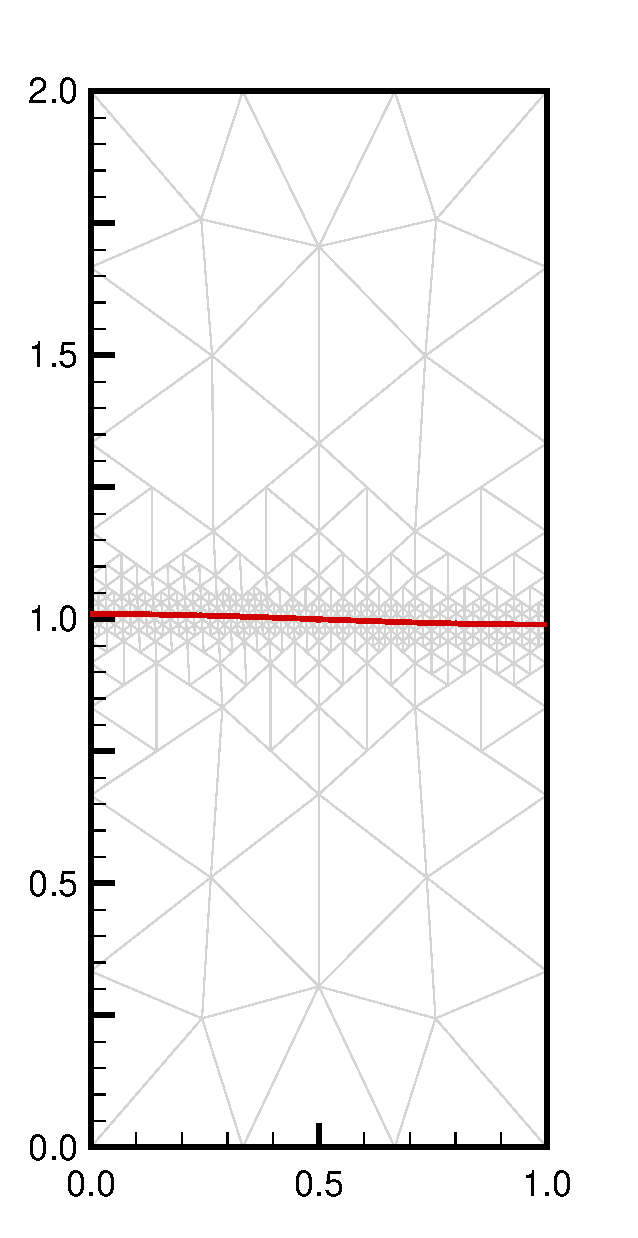
\includegraphics[width=\textwidth]{StandingWave_N3_a01_full.eps}
				%				\label{Fig:StandingWaveMeshSmall_Global}
				\caption{}
			\end{subfigure}
			~
			\begin{subfigure}[]{0.25\textwidth}
				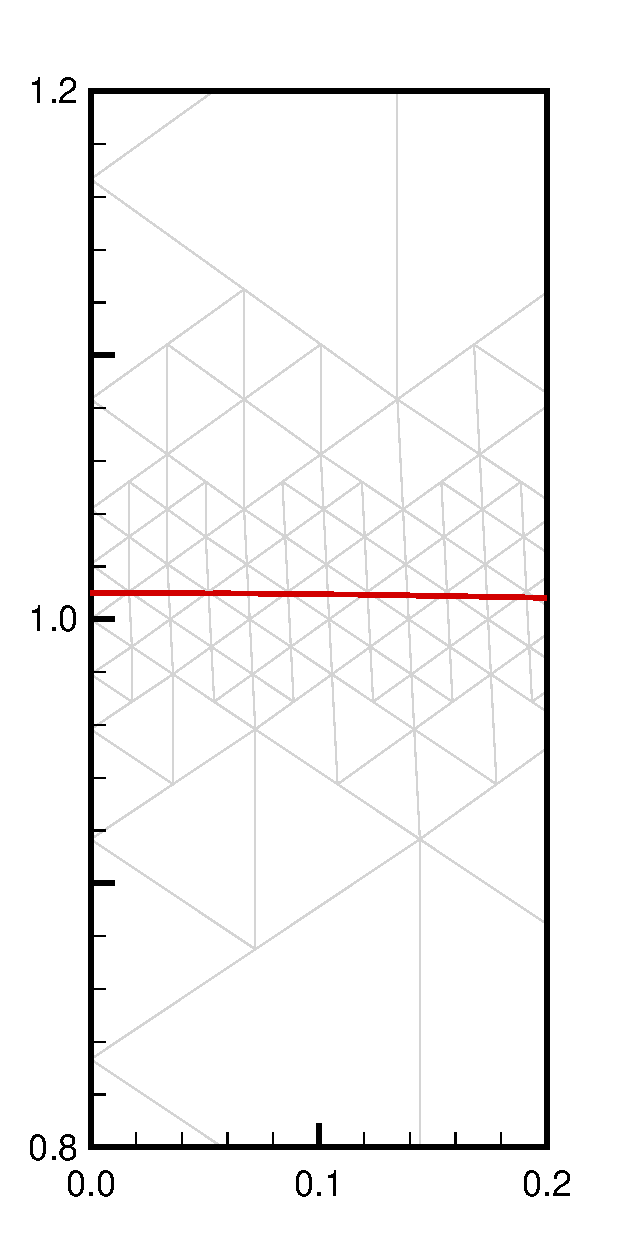
\includegraphics[width=\textwidth]{StandingWave_N3_a01_zoom.eps}
				%					\label{Fig:StandingWaveMeshSmall_Zoomed}
				\caption{}
			\end{subfigure}
			~
			\begin{subfigure}[]{0.45\textwidth}
				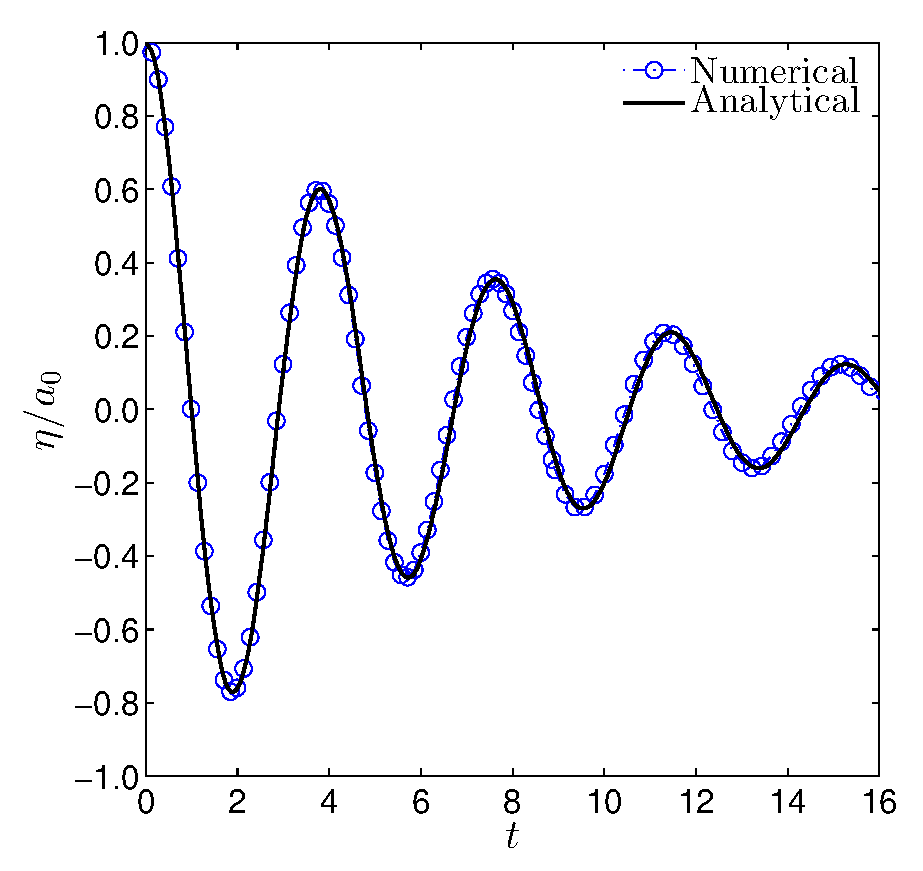
\includegraphics[width=\textwidth]{StandingVaweAmplitudeExact.eps}
				%									\label{Fig:StandingWave_WavelengthSmall_d}
				\caption{}
			\end{subfigure}
		\end{center}
		\caption{(\textcolor{red}{TODO}: Bastirinca ag cizgileri net gorunmuyor)Sloshing problem for the small amplitude case, (a) Computational grid and  initial interface shape for $ l_{M} = 3 $ (b) Zoomed view  near the left wall. (c) Comparison of the computed wave amplitude with analytical solution \cite{wu_effect_2001}. ($ \rho_l/\rho_g  = 100$, $ \mu_l/\mu_g  = 100$,  $ Re = 100 $ (\textcolor{red}{TODO}: Bu Re hangi ozellikleri kullanarak hesaplandi?),  $ Fr = 1 $, $ N=3 $, $ a_0 = 0.01 $ )}
		\label{Fig:StandingWaveMeshSmall}
	\end{figure}
	%%
	
	The problem is first solved in the computational domain of $ [0,d]\times [0,2d] $ for the small amplitude, $ a_0 = 0.01$, where an analytical solution based on the linearized Navier-Stokes equations is reported by Wu et.al. \cite{wu_effect_2001}. The initial grid has elements with a characteristic element length of $ h=1/3 $ ($ K=50 $), which is refined adaptively near $ y=1 $ with $l_{M}=3$ as shown in \aref{Fig:StandingWaveMeshSmall}(a-b) (\textcolor{red}{TODO}: Cumleyi degistirdim. Bunu mu demek istemistin? Normal bir adaptive mesh cozumu degil mi bu?). Slip boundary condition is assigned to the bottom and side walls while zero pressure is imposed at the top wall. Zero velocities and hydrostatic pressure distribution are used as the initial condition. Density and viscosity ratios of the liquid and gas phases are both $ 100 $. The non-dimensional Froude and Reynolds numbers are taken as $ 1 $ and $ 100 $ (\textcolor{red}{TODO}: Bu Re sayisinin hangi mu, rho, U ve L ile hesaplandigi belli degil), respectively. \aref{Fig:StandingWaveMeshSmall}(c) shows variation of the normalized wave elevation, $ \eta/a_0 $ in time for computed and analytical solutions. Numerical result matches well with the analytical one.
	%For this flow,  $ U_r =\sqrt{gd}$ is taken  as a reference value for the velocity, $ L_R = d $ is the reference length.
	%%
	
	\aref{Fig:StandingWave_N5_a2} shows the $ l_M = 3 $ locally adapted mesh structures and interfaces at different simulation times for the high initial amplitude case with $ a_0 = 0.2 $. Polynomial order is set to $5$ and all other parameters are kept the same as the previous low apmplitude solution. Time integration is carried out until $ t =40 $, where the liquid column comes to rest. Mesh adaptivity used here always keeps the interface in the highest refinement level elements. Letting the number of hanging nodes per face unconstrained (\textcolor{red}{TODO}: 3:1 oranina ne oldu?) enables us to get the desired local mesh refinement (\textcolor{red}{TODO}: Bu cumle kalkabilir).
	%%
	\begin{figure}[ht!]
		\begin{center}
			\begin{subfigure}[]{0.2\textwidth}
				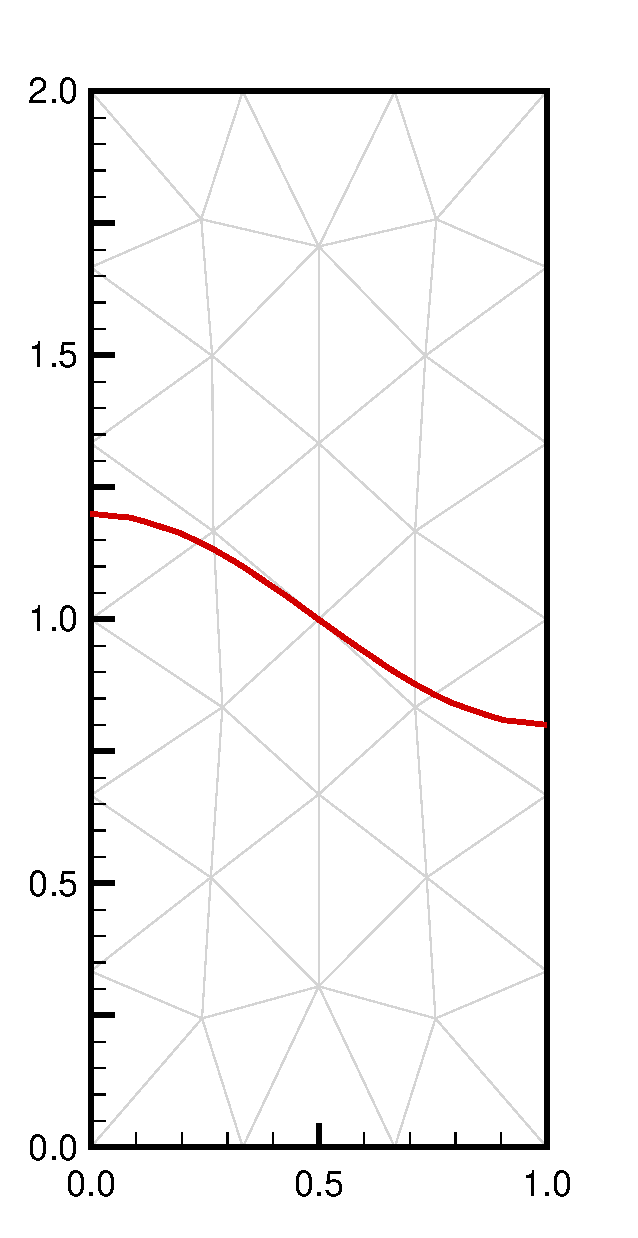
\includegraphics[width=\textwidth]{SW_N5_L3_0.eps}
				%			\label{Fig:StandingWave_N3_a2_L0}
				\caption{$ t = 0 $}
			\end{subfigure}
			~
			\begin{subfigure}[]{0.2\textwidth}
				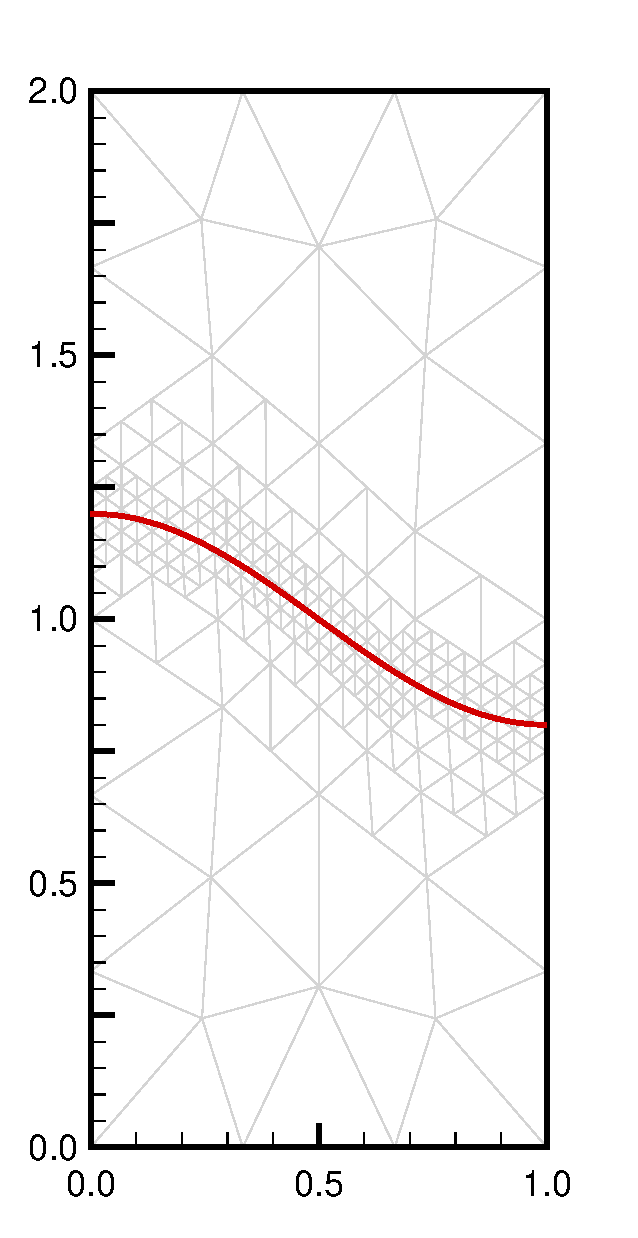
\includegraphics[width=\textwidth]{SW_N5_L3_1.eps}
				%			\label{Fig:StandingWave_N3_a2_L0}
				\caption{$ t = 0 $}
			\end{subfigure}
			%		~
			%		\begin{subfigure}[]{0.23\textwidth}
			%			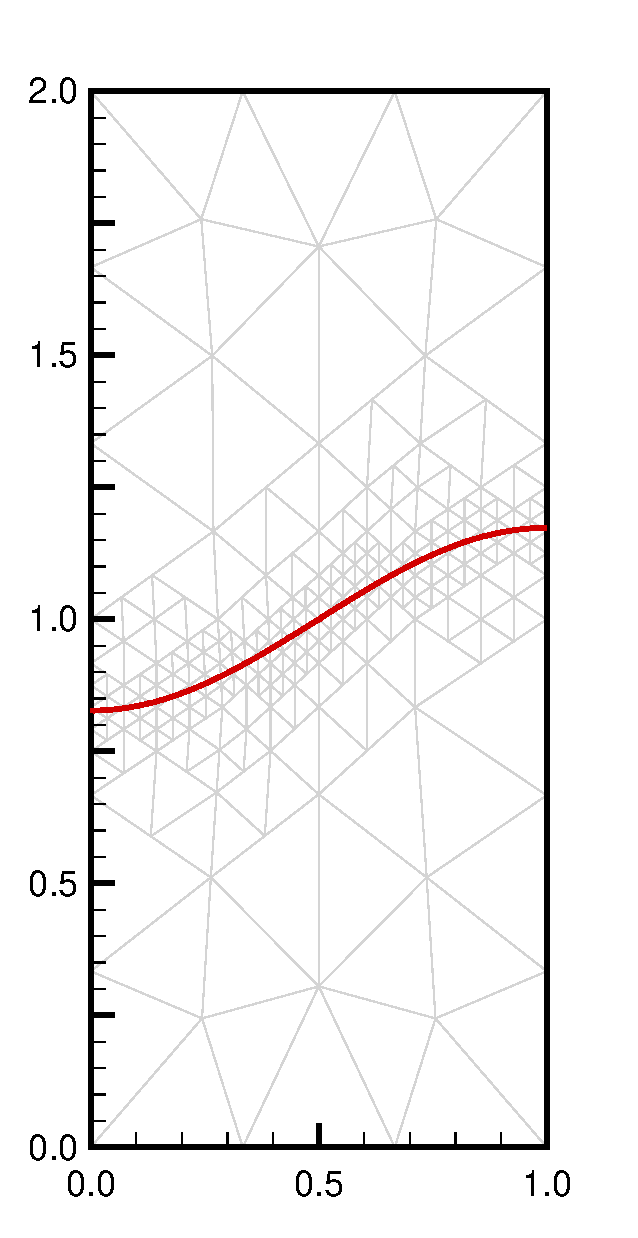
\includegraphics[width=\textwidth]{SW_N5_L3_2.eps}
			%%			\label{Fig:StandingWave_N3_a2_L1}
			%			\caption{$ t = 2.2 $}
			%		\end{subfigure}
			%		~
			%		\begin{subfigure}[]{0.23\textwidth}
			%			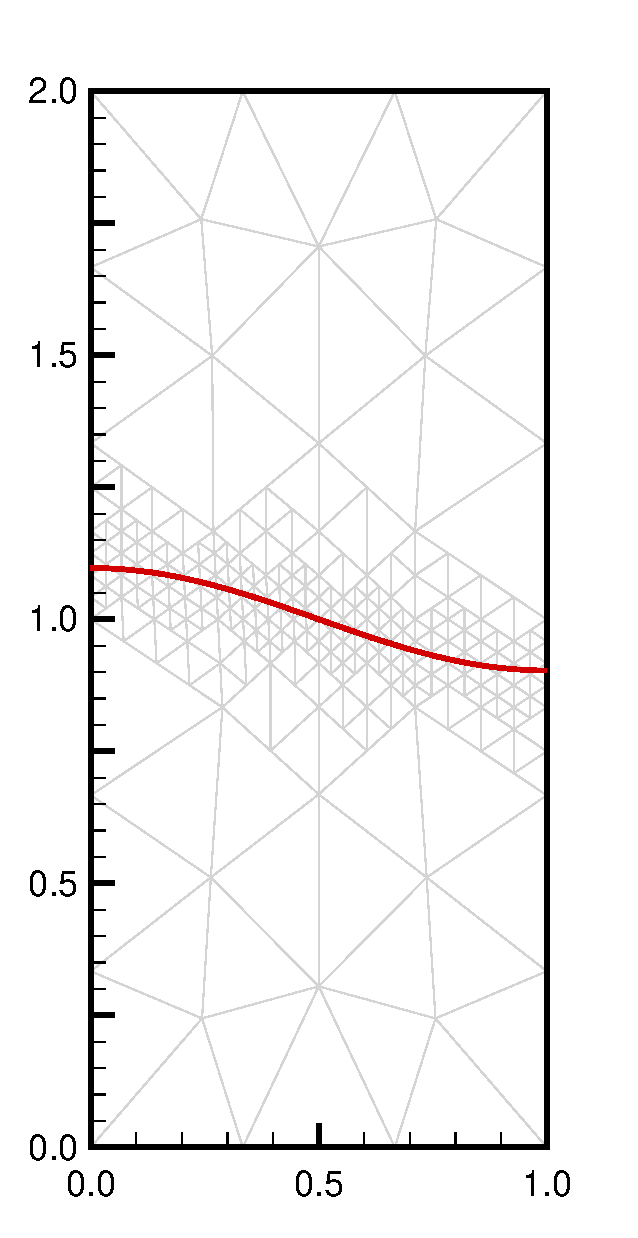
\includegraphics[width=\textwidth]{SW_N5_L3_3.eps}
			%%			\label{Fig:StandingWave_N3_a2_L2}
			%			\caption{$ t = 9.2 $}
			%		\end{subfigure}
			%		~
			%		\begin{subfigure}[]{0.23\textwidth}
			%			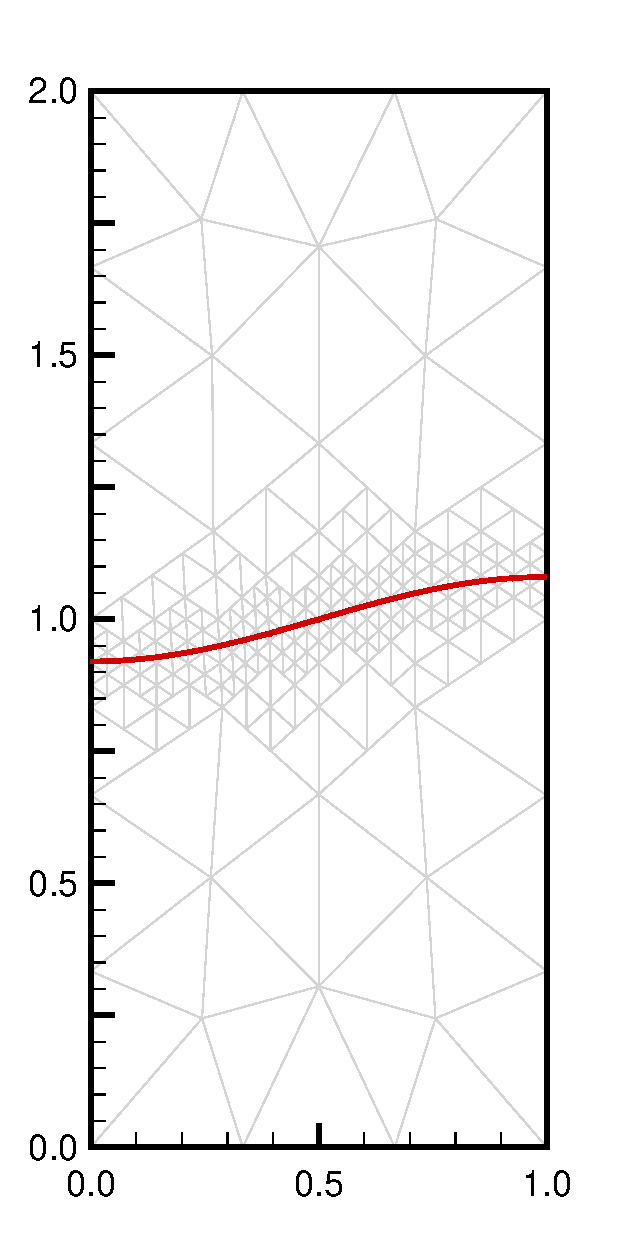
\includegraphics[width=\textwidth]{SW_N5_L3_4.eps}
			%%			\label{Fig:StandingWave_N3_a2_L3}
			%			\caption{$ t = 11.5$}
			%		\end{subfigure}
			%			~
			%		\begin{subfigure}[]{0.23\textwidth}
			%				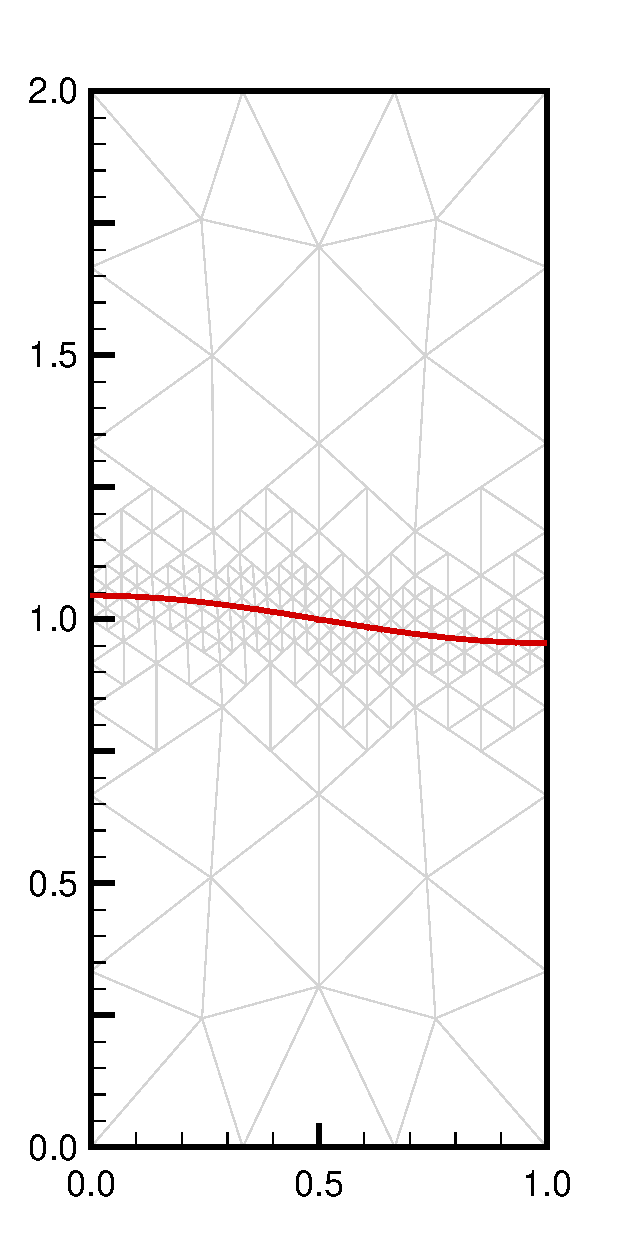
\includegraphics[width=\textwidth]{SW_N5_L3_5.eps}
			%%				\label{Fig:StandingWave_N3_a2_L2}
			%				\caption{$t=18.6 $}
			%		\end{subfigure}
			%			~
			\begin{subfigure}[]{0.2\textwidth}
				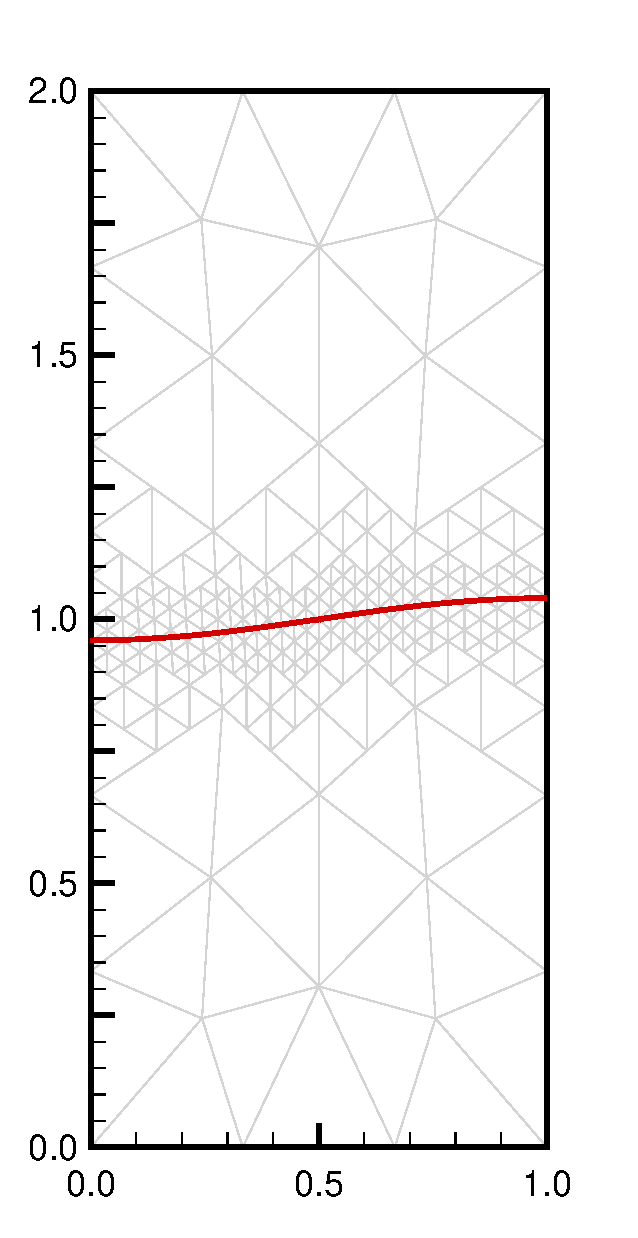
\includegraphics[width=\textwidth]{SW_N5_L3_6.eps}
				%				\label{Fig:StandingWave_N3_a2_L3}
				\caption{$ t =20.5 $}
			\end{subfigure}
			~
			\begin{subfigure}[]{0.2\textwidth}
				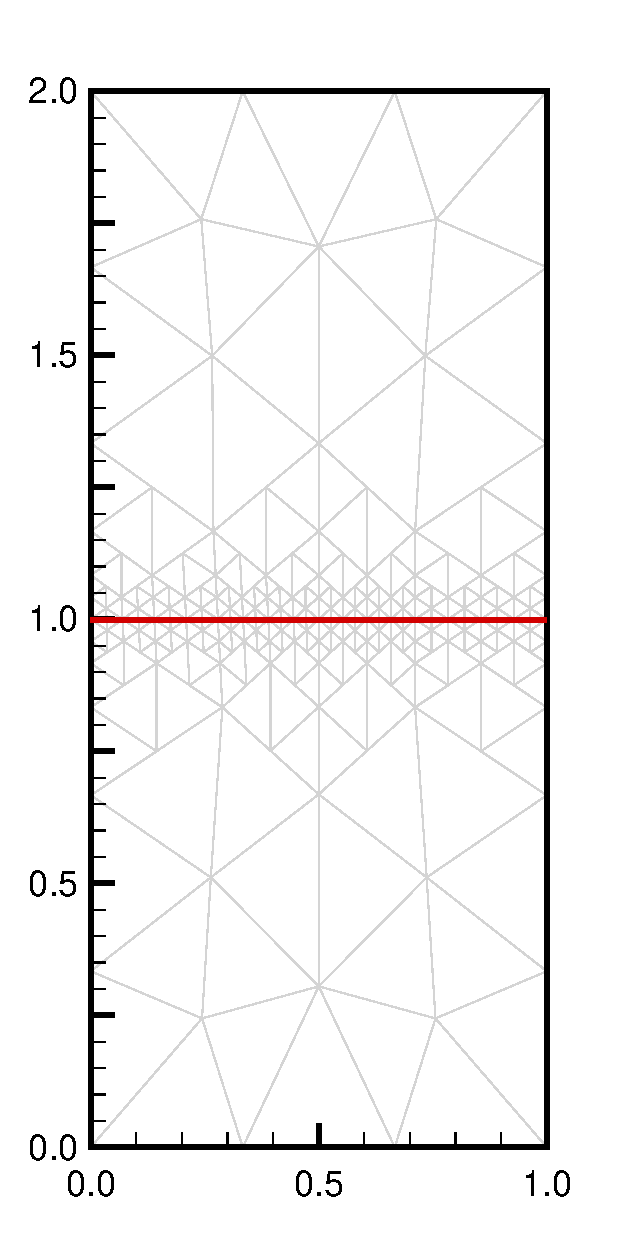
\includegraphics[width=\textwidth]{SW_N5_L3_7.eps}
				%				\label{Fig:StandingWave_N3_a2_L3}
				\caption{$t =40$}
			\end{subfigure}
		\end{center}
		\caption{(\textcolor{red}{TODO}: Bastirinca ag cizgileri net gorunmuyor)$ l_M = 3 $ locally adapted grid and the interface at different simulation times for the high amplitude sloshing. ($ \rho_l/\rho_g  = 100$, $ \mu_l/\mu_g  = 100$,  $ Re = 100 $,  $ Fr = 1 $, $ N=5 $, $ a_0 = 0.2 $ )}
		\label{Fig:StandingWave_N5_a2}
	\end{figure}
	%%
	
	\Aref{Table:StandingWaveAreaLoss} shows the liquid phase (\textcolor{red}{TODO}: Ben ekledim, dogru mu?) mass fluctuations introduced by the scheme for long time integration. Different refinement levels and order of approximations are used in the numerical experiments. Mass fluctuations are computed very accurately by the adaptive contouring algorithm (\textcolor{red}{TODO}: Nedir bu contouring algorithm? refinement algorithm mi demek istiyorsun?) using the formula, $ A_f =100\times (\max(A_t)- \min(A_t)) / A_{exact} $, where $ A_t $ is the time history of the area of the liquid phase. Mass is well conserved for this long time integration solution and increasing resolution in the vicinity of interface significantly improves it. 
	% 
	\begin{table}[ht]
		\caption{Percentage mass fluctuations of the liquid phase for the sloshing problem obtained using different refinement levels and approximation orders.}
		\centering
		\label{Table:StandingWaveAreaLoss}
		\small\addtolength{\tabcolsep}{5pt}
		\begin{tabular}{p{2cm} p{2cm}  p{2cm} p{2cm} p{2cm} }
			%	\begin{tabular}{ c c c c c }
			\hline \hline
			&    &  \multicolumn{3}{ c }{$ l_{M} $}  \\ \cline{3-5} 
			&\multicolumn{1}{c}{ $ N $ }    &  0           & 1           & 2          \\  \hline\hline
			%\multirow{3}{*}{ $ \% $ Mass Fluctuation}&\multicolumn{1}{c}{ 2 }   & -            & -          &  -         \\
			\multirow{3}{*}{ $ \% $ Mass Fluctuation} & \multicolumn{1}{c}{ 3 } & $ 4.52\times 10^{-1}$       & $ 1.11\times 10^{-1}$     &  $ 2.12\times 10^{-2}$       \\
			& \multicolumn{1}{c}{ 4 }       & $ 1.51\times 10^{-1}$        & $ 8.27\times 10^{-2}$     &  $ 6.60\times 10^{-3}$       \\
			& \multicolumn{1}{c}{ 5}        & $ 6.33\times 10^{-2}$        & $ 1.55\times 10^{-2}$     &  $ 2.01\times 10^{-3}$      \\ \hline \hline	
		\end{tabular}
	\end{table}
	%%
	
	
	%\subsection{Dam Break Problem}
	%Dam break problem consists of sudden collapse of a rectangular liquid column into a horizontal plane under the action of gravitational acceleration. Flow field is highly unsteady and interface encounters strong deformations. Due to viscosity, water column eventually comes to rest and occupy the bottom of the tank. Measurements of the exact interface shape and analytical solution for the viscous case are not available but some secondary data such as column height reduction and wave front speeds are reported in literature.   
	%%
	%
	%%To compare the present numerical method with the experimental data reported by Martin and Moyce \cite{martin_part_1952}, 
	%All computations are conducted on the $ [0,1.5a]\times [0,6a] $ domain with $ a = 1 $. Square water column with the length of $ a $  is released at $ t = 0 $. Slip boundary conditions are applied to the bottom and side walls of the tank. Similar to the experimental study, top wall is modeled as open boundary with zero atmospheric pressure and zero normal gradients on the velocities. Water and air properties are assigned to the liquid and gas phases as  $\rho_l = 1000\;\text{kg}\;\text{m}^{-3}  $, $\rho_g = 1\;\text{kg}\;\text{m}^{-3} $ and $\mu_l = 10^{-3}\;\text{Pa}\;\text{s}  $, $\mu_g = 10^{-5}\;\text{Pa}\;\text{s}$. Selecting the characteristic length, $ L_R = 0.05715\;\text{m} $ and using the properties given, corresponding  non-dimensional Reynolds and Froude numbers are $ 42792 $ and $  1 $, respectively.
	%%
	%
	%\begin{figure}[ht!]
	%	\begin{center}
	%		\begin{subfigure}[]{0.45\textwidth}
	%			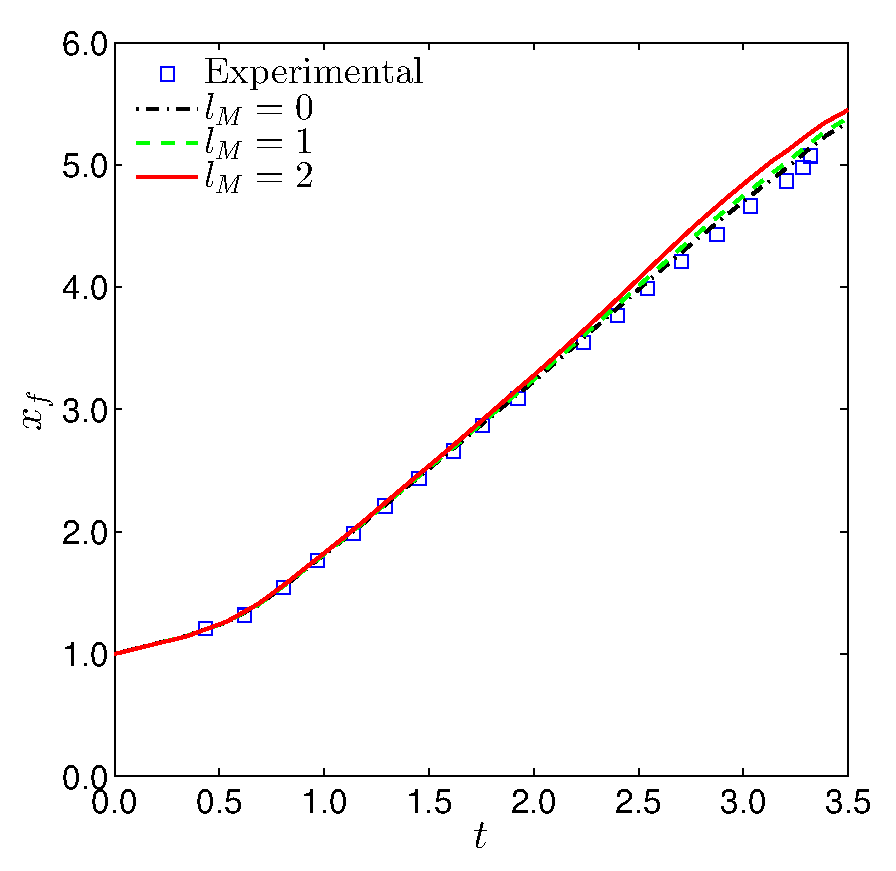
\includegraphics[width=\textwidth]{DamBreakSurgeFront.eps}
	%			%				\label{Fig:StandingWaveMeshSmall_Global}
	%			\caption{Surge front position}
	%		\end{subfigure}
	%		~
	%		\begin{subfigure}[]{0.45\textwidth}
	%			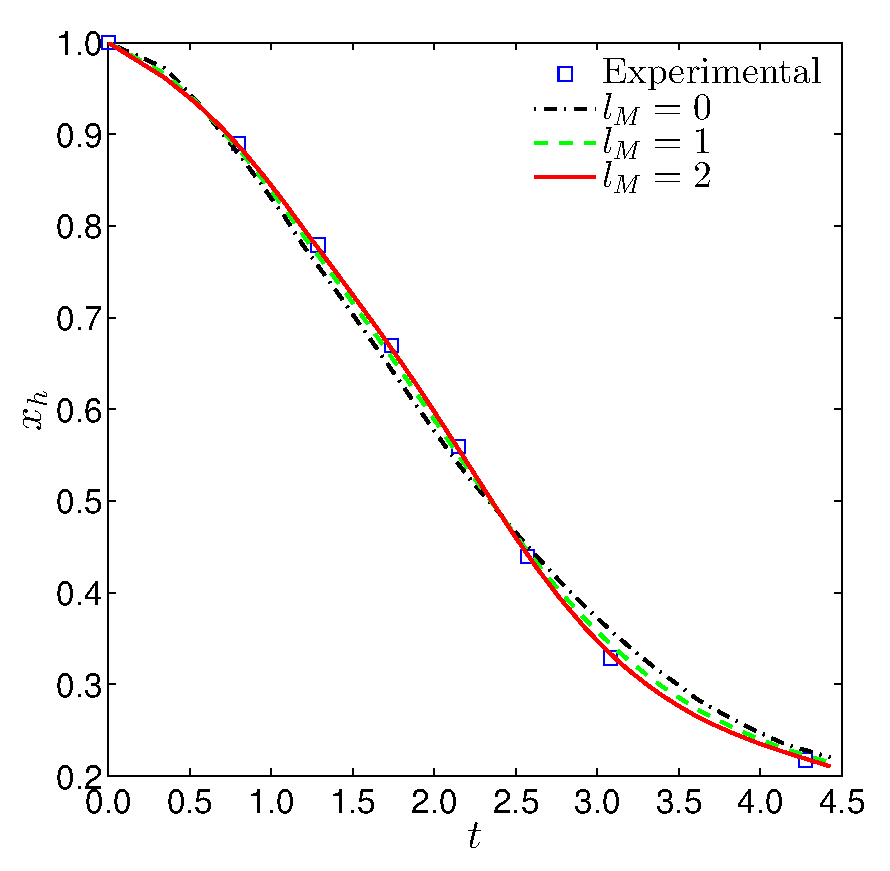
\includegraphics[width=\textwidth]{DamBreakColumnHeight.eps}
	%			%					\label{Fig:StandingWaveMeshSmall_Zoomed}
	%			\caption{Water column height}
	%		\end{subfigure}
	%	\end{center}
	%	\caption{Comparison of the present numerical method with different refinement levels and experimental results from  Martin and Moyce \cite{martin_part_1952}. ($ Re = 3000 $,  $ Fr = 1 $, $ N=3 $)}
	%	\label{Fig:DamBreakComparasion}
	%\end{figure}
	%
	%\Aref{Fig:DamBreakComparasion} shows the comparison between the numerically computed surge front position and water column height and experimental results reported by  Martin and Moyce \cite{martin_part_1952}. Initial coarse grid has the  characteristic length, $ h=1/4 $ which gives $ K=172 $. Local polynomial order of $ 3 $ is used in all simulations. Increasing the adaptive level, non-dimensional height of the water column corresponds very well with the experimental data. Numerical results show that surge front position moves faster when the resolution near the interface increased. A thin fluid layer forms at the bottom wall just in front of the bulk flow and adaptive contouring algorithm accurately locate the position of the front according to the thin layer. Difficulty to determine the exact location of the leading edge position is confirmed in experimental study \cite{martin_part_1952} and the same tendency is shown in other numerical works \cite{ubbink_1999,kelecy_development_1997}.    
	%%%
	%
	%\begin{figure}[ht!]
	%	\begin{center}
	%		\begin{subfigure}[]{0.85\textwidth}
	%			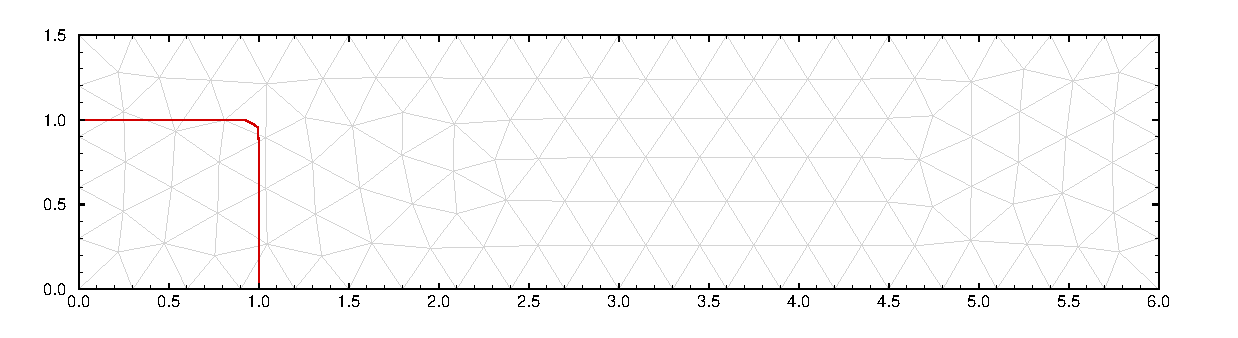
\includegraphics[width=\textwidth]{DB_L0_Inter_t_0.eps}
	%			%				\label{Fig:StandingWaveMeshSmall_Global}
	%			\caption{Coarse grid, $ t=0 $}
	%		\end{subfigure}
	%		~
	%		\begin{subfigure}[]{0.85\textwidth}
	%			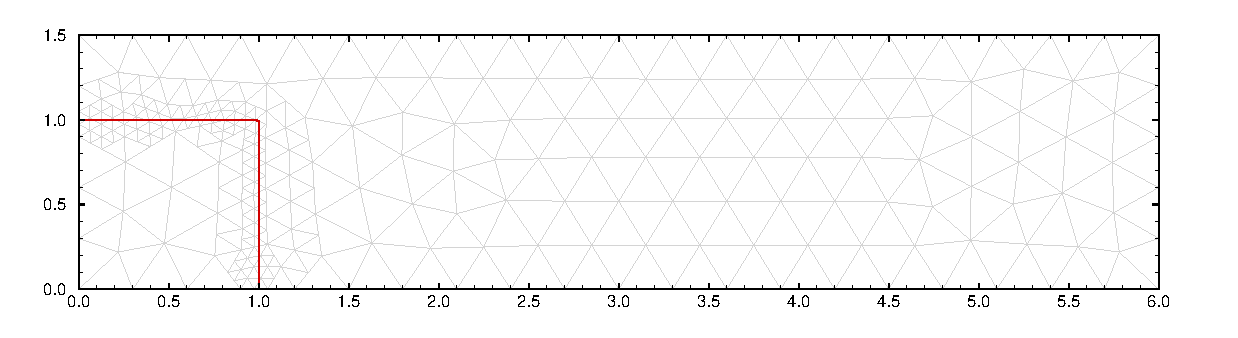
\includegraphics[width=\textwidth]{DB_L2_Inter_t_0.eps}
	%			%				\label{Fig:StandingWaveMeshSmall_Global}
	%			\caption{$ l_M = 2 $ adaptive grid, $ t = 0 $}
	%		\end{subfigure}
	%		~
	%		\begin{subfigure}[]{0.85\textwidth}
	%			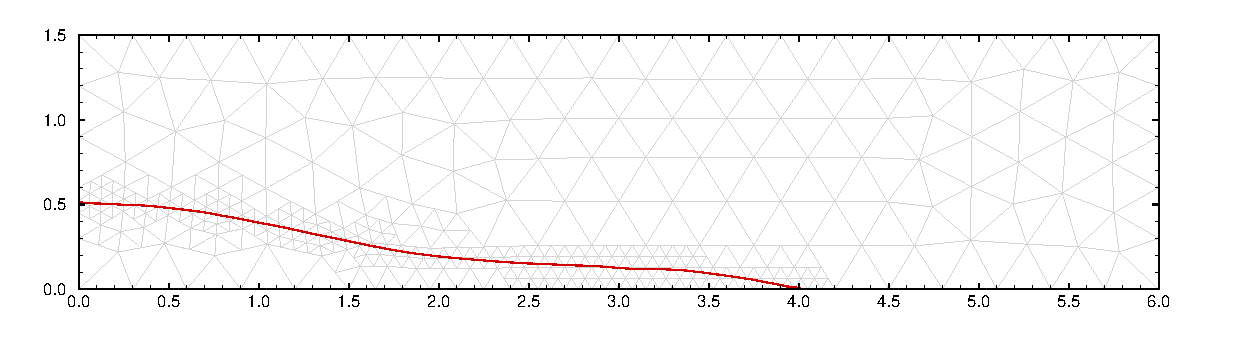
\includegraphics[width=\textwidth]{DB_L2_Inter_t_2_5.eps}
	%			%				\label{Fig:StandingWaveMeshSmall_Global}
	%			\caption{$ l_M = 2 $ adaptive grid, $ t = 2.5 $}
	%		\end{subfigure}
	%		~
	%		\begin{subfigure}[]{0.85\textwidth}
	%			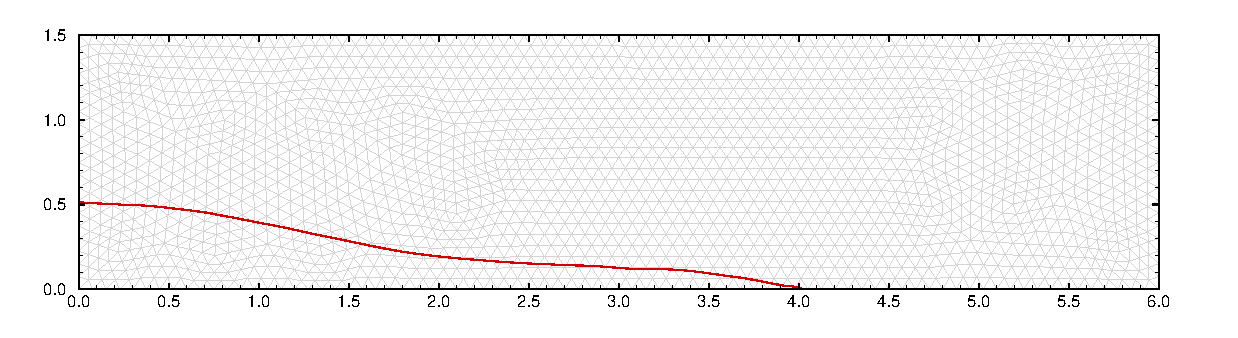
\includegraphics[width=\textwidth]{DB_F2_Inter_t_2_5.eps}
	%			%				\label{Fig:StandingWaveMeshSmall_Global}
	%			\caption{Fixed grid, $ t = 2.5 $}
	%		\end{subfigure}
	%	\end{center}
	%	\caption{Dam break problem interface locations and mesh structures. ($ Re = 42792 $,  $ Fr = 1 $, $ N=3 $)}
	%	\label{Fig:DamBreakInterface}
	%\end{figure}
	%%%
	%
	%\Aref{Fig:DamBreakInterface} illustrates the interface shapes and mesh structures. (a) and (b) show initial coarse grid and interface for $ K = 242 $,  $ N=3 $ and Lagrange interpolation of the initial data  to  $ l_M = 2 $ locally adapted grid, respectively.  (c-d) represents the interface at $ t = 2.5 $ for adaptive simulation and  $ 2 $ level globally refined fixed grid. A careful investigation of the figure  reveals the consistency of adaptive simulation where varying mesh resolution and non-conformal discretization do not degenerate the accuracy near the interface. It is worthwhile to mention that total number of elements in fixed grid  is $ 3904 $ and adaptive grid has $ 610$ elements at that instant. Computational effort is significantly reduced to obtain the same accuracy with fixed grid.   
	%%%%
	%% 
	%%\begin{table}[ht]
	%%	\caption{Percentage mass fluctuations in dam break problem for different refinement levels and order of approximations. }
	%%	\centering
	%%	\label{Table:DamBreakAreaLoss}
	%%	\small\addtolength{\tabcolsep}{5pt}
	%%%	\begin{tabular}{p{2cm} p{2cm}  p{2cm} p{2cm} p{2cm} }
	%%	\begin{tabular}{ c c c c c }
	%%	\hline \hline
	%%$ l_M $	                &  $ N $   &  $  A_l $ $ (t =1.5) $ &   $ A_l $ $ (t =3.0) $ &    $ A_l $ $ (t =4.5) $  \\   \hline\hline
	%%\multirow{2}{*}{$ 0 $}	&    3     & 1                      &     1                  &    1            \\ 
	%%%                    	&    4      & 1                      &     1                  &    1            \\
	%%                    	&    5      & 1                      &     1                  &    1            \\ \cline{2-5}	
	%%\multirow{2}{*}{$ 1 $}	&    3     & 1                      &     1                  &    1            \\ 
	%%%                    	&    4      & 1                      &     1                  &    1            \\
	%%                        &    5      & 1                      &     1                  &    1            \\	\cline{2-5}
	%%\multirow{2}{*}{$ 2 $}	&    3     & 1                      &     1                  &    1            \\ 
	%%%                    	&    4      & 1                      &     1                  &    1            \\
	%%                        &    5      & 1                      &     1                  &    1            \\	\hline\hline                    	
	%%	\end{tabular} 
	%%\end{table}
	%%%%
	%%
	%%Percentage area loss of the dam break problem for  different refinement levels and order of approximations at $ t =1.5 $, $ t =3.0 $ and $ t =4.5 $ are given in Table.\ref{Table:DamBreakAreaLoss}.  
	
	
	\subsection{Rayleigh-Taylor instability}
	In this commonly used test problem a heavy fluid overlies a lighter one. Instability arises when the initial interface is perturbed. Due to the vertical gravitational field, fluids start penetrating into each other with increasing amplitude in time. Problem is solved in the 2D rectangular domain of $ [0,d/2]\times [0,4d] $, with the characterisitic length $d$ being $...$ (\textcolor{red}{TODO}: Degeri nedir?). Boundary conditions are slip at the side walls, no-slip at the bottom wall and prescribed zero pressure at the top wall. Initial conditions are taken as zero velocity field and hydrostatic pressure distribution. Interface between the fluids is initially perturbed with a cosine function of amplitude $ 0.1 $ , $ \eta = 2.0 + 0.1\cos(2\pi x) $ (\textcolor{red}{TODO}: 2 degeri 2d'ye mi esit? Oyle mi yazmali?). Dynamic viscosities of the fluids are equal and their density difference is given by the Atwood ratio, $ \text{At} = (\rho_l - \rho_g)/ ( \rho_l + \rho_g)$. To use the same notation with \cite{tryggvason_numerical_1988}, reference time is chosen as $ t_r = \sqrt{d/(g\text{At})} $ (\textcolor{red}{TODO}: bu neyi hesaplamak icin gerekiyor ki? Makalede baska bir yerde geciyor mu?).
	
	%%
	\begin{figure}[ht!]
		\begin{center}
			\begin{subfigure}[]{0.35\textwidth}
				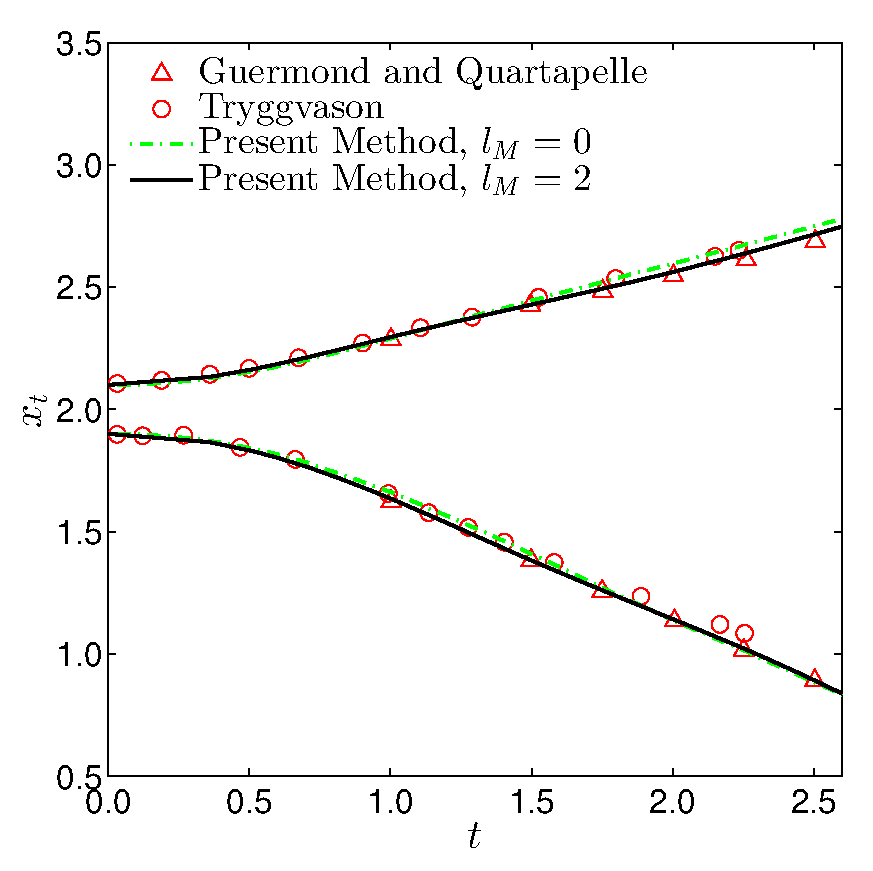
\includegraphics[width=\textwidth]{RayleighTaylorTipPosition.eps}
			\end{subfigure}
		\end{center}
		\caption{(\textcolor{red}{TODO}. Kesikli cizgi net gorunmuyor bastirinca. Legend'daki referans cozumlere referans numarasi konmali)Tip positions of the rising and dropping fluids for Rayleigh Taylor instability. ($ \text{Re} = 42792 $,  $ \text{At} = 0.5 $, $ N=3 $)}
		\label{Fig:RayleighTaylorComparasion}
	\end{figure}
	%
	%
	%%%
	%\begin{figure}[ht!]
	%	\begin{center}
	%	\begin{subfigure}[]{0.15\textwidth}
	%		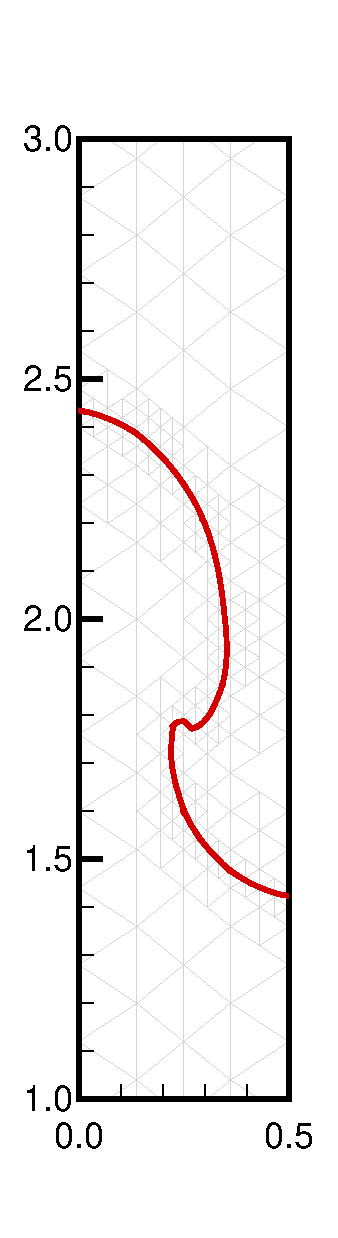
\includegraphics[width=\textwidth]{RT_Inter_Adapt.eps}
	%     \end{subfigure}
	%     \end{center}
	%	\caption{Tip positions of the rising and dropping fluids for Rayleigh Taylor instability. ($ \text{Re} = 42792 $,  $ \text{At} = 0.5 $, $ N=3 $)}
	%	\label{Fig:RayleighTaylorAdapt}
	%\end{figure}
	%%
	
	Non-dimensional tip positions of the rising and dropping fluid columns, $ x_t $ (\textcolor{red}{TODO}: Dusey uzunluk oldugu icin $ y_t $ daha iyi mi olur? Degisirse figurde de degismeli) are given in \aref{Fig:RayleighTaylorComparasion} for $ \text{Re} =  \rho_l d^{3/2}g^{1/2}/ \mu_l = 3000 $ (\textcolor{red}{TODO}: Fig. 3'teki rakam 3000 degil. Sonraki figurde 3000.) and $ \text{At} = 0.5 $. For comparison, results obtained by the Lagrangian-Eulerian vortex method \cite{tryggvason_numerical_1988} and the variable density finite element projection method \cite{guermond_projection_2000} are also included. Numerical results are obtained for a fixed grid with characteristic length $ h=1/3 $ $( K=212 )$ and locally adapted grid with $l_M = 2 $. As seen, present results compare well with the previous works and increasing resolution near the interface improves the accuracy.
	
	%%
	\begin{figure}[ht!]
		\begin{center}
			\begin{subfigure}[]{0.1\textwidth}
				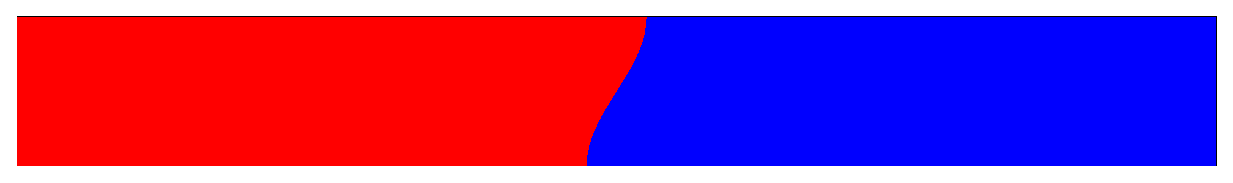
\includegraphics[trim=150 0 100 0,clip,angle=-90,origin=c,width=\textwidth]{RT_Cont_1.eps}
				\caption{}
			\end{subfigure}
			~
			\begin{subfigure}[]{0.1\textwidth}
				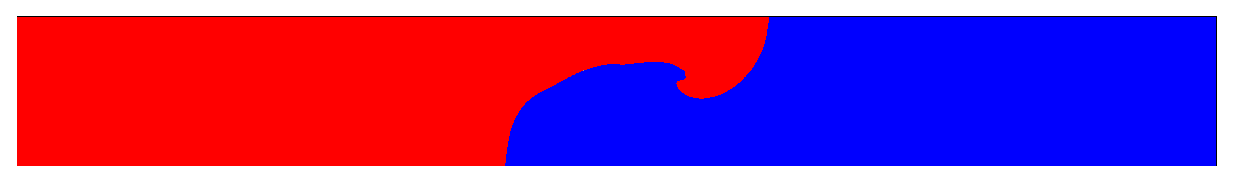
\includegraphics[trim=150 0 100 0,clip,angle=-90,origin=c,width=\textwidth]{RT_Cont_50.eps}
				\caption{}
			\end{subfigure}
			~
			\begin{subfigure}[]{0.1\textwidth}
				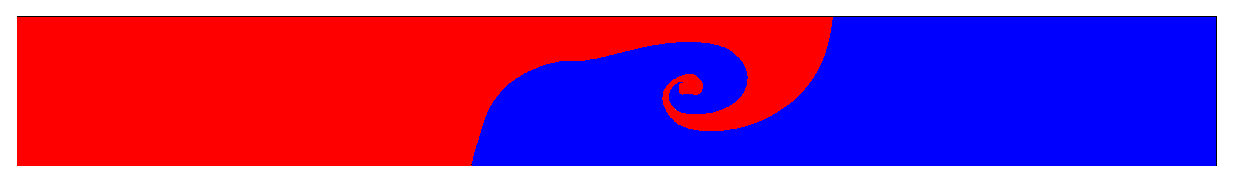
\includegraphics[trim=150 0 100 0,clip,angle=-90,origin=c,width=\textwidth]{RT_Cont_75.eps}
				\caption{}
			\end{subfigure}
			~
			\begin{subfigure}[]{0.1\textwidth}
				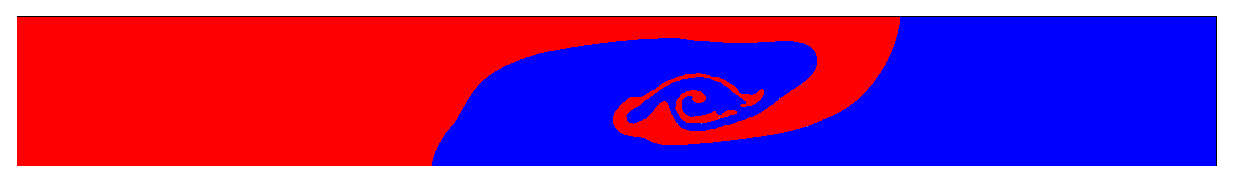
\includegraphics[trim=150 0 100 0,clip,angle=-90,origin=c,width=\textwidth]{RT_Cont_110.eps}
				\caption{}
			\end{subfigure}
			~
			\begin{subfigure}[]{0.1\textwidth}
				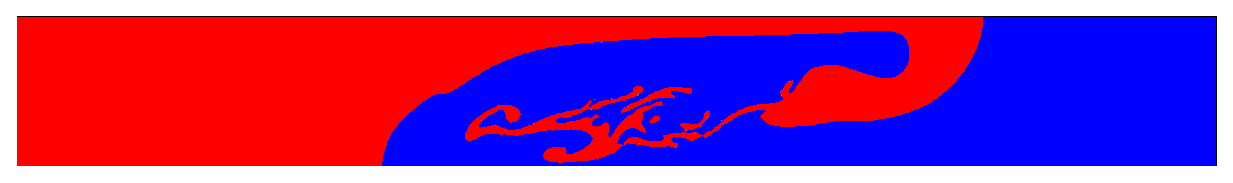
\includegraphics[trim=150 0 100 0,clip,angle=-90,origin=c,width=\textwidth]{RT_Cont_156.eps}
				\caption{}
			\end{subfigure}
		\end{center}
		\caption{(\textcolor{red}{TODO}: Bir onceki figurde N=3 idi, bunda ise N=5. Dogru mu bunlar?. Basilinca kontrast'tan dolayi zor ayriliyor iki faz? Kontrast artirilabilir kullanilan renklerde.)Interface evolution of the Rayleigh-Taylor instability for  $ l_M = 2 $ adaptive solution at $ t = 0 $, $ 1.28 $,  $ 1.71 $,  $ 2.18 $, $2.70$ ($ \text{Re} = 3000 $,  $ \text{At} = 0.5 $, $ N=5 $. Only a part of the domain is shown).}
		\label{Fig:RayleighTaylorInterface}
	\end{figure}
	%%
	%%%
	\begin{figure}[ht!]
		\begin{center}
			\begin{subfigure}[]{0.15\textwidth}
				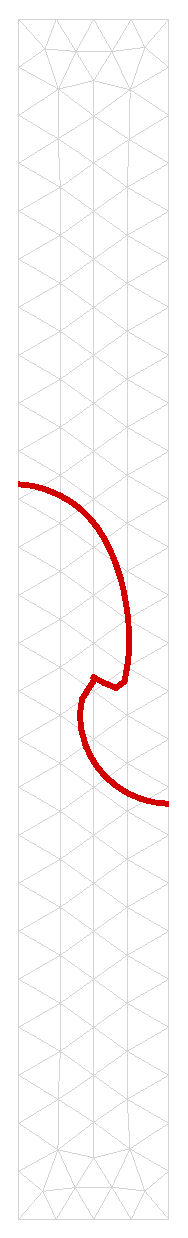
\includegraphics[trim=0 180 0 200,clip,width=\textwidth]{RT_L0_N3.eps}
				\caption{}
			\end{subfigure}
			~
			\begin{subfigure}[]{0.15\textwidth}
				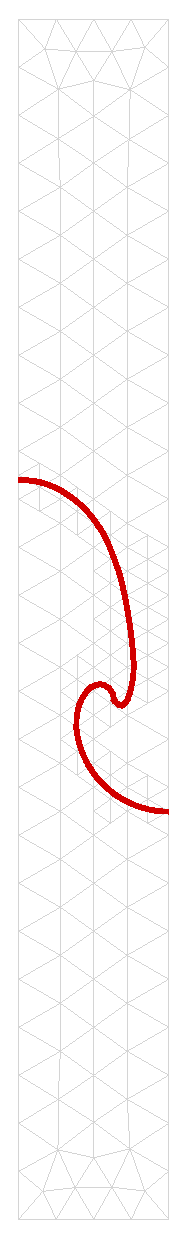
\includegraphics[trim=0 180 0 200,clip,width=\textwidth]{RT_L1_N3.eps}
				\caption{}
			\end{subfigure}
			~
			\begin{subfigure}[]{0.15\textwidth}
				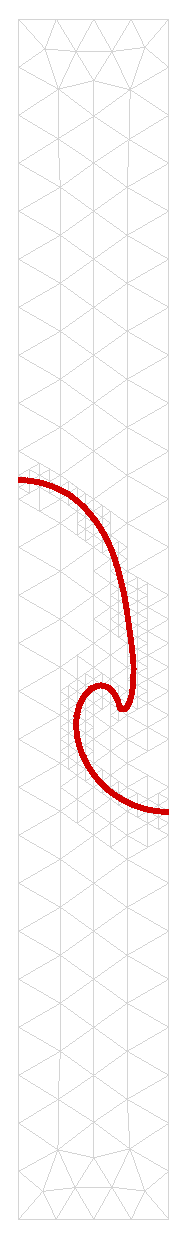
\includegraphics[trim=0 180 0 200,clip,width=\textwidth]{RT_L2_N3.eps}
				\caption{}
			\end{subfigure}
		\end{center}
		\caption{Interface shapes of the Rayleigh-Taylor instability for (a) fixed grid (b) $ l_M = 1 $ and (c) $ l_M = 2 $ locally adapted grids ($ t = 1.63 $, (\textcolor{red}{TODO}: Yazi icinde 1.163 yaziyordu, ben kaldirdim o cumleyi. O mu dogruydu bu mu?) $ \text{Re} = 500 $,  $ \text{At} = 0.5 $, $ N=3 $. Only a part of the domain is shown).}
		\label{Fig:RayleighTaylorAdaptiveInterface}
	\end{figure}
	%%
	
	
	\Aref{Fig:RayleighTaylorInterface} shows the interface shapes for $ l_M =2 $ locally adapted grid at different simulation times. Results compare well with those reported by Puckett et al. \cite{puckett_high-order_1997}, Popinet and Zaleski \cite{popinet_front-tracking_1999} and Xie et al.\cite{xie_adaptive_2014}. Mesh adaptation details for $ \text{Re} = 500 $ solution are shown in \aref{Fig:RayleighTaylorAdaptiveInterface}. Effective local adaptation of the initial coarse mesh around the complext interface is clearly seen. At the shown instant, element numbers of the fixed and the adpated grids with $ l_M = 1 $ and $ l_M = 2 $ are $ \textcolor{red}{TODO}: Fixed grid'deki eleman sayisini yaz$, $ 305 $ and $ 425 $, respectively. 
	%
	
	\begin{table}[ht]
		\caption{Percentage mass fluctuations of the liquid phase of the Rayleigh-Taylor instability problem for different refinement levels and approximation orders ($ \text{Re} = 500 $,  $ \text{At} = 0.5 $).}
		\centering
		\label{Table:RayleighTaylorAreaLoss}
		\small\addtolength{\tabcolsep}{5pt}
		\begin{tabular}{ c  c c c c  }
			\hline \hline 
			Method                          &   $ l_M $	                &  $ N $   &  Element Number   &  $ \% $ Mass Loss   \\   \hline\hline
			\multirow{8}{*}{Present Method}    &  \multirow{4}{*}{$ 0 $}	&    3     &   $ 212 $         & 0.259            \\
			&                           &    5     &   $ 212 $         & 0.148            \\ 
			&                           &    3     &   $ 836 $         & 0.093            \\ 
			&                           &    5     &   $ 836 $         & 0.032            \\ \cline{3-5}	
			& \multirow{2}{*}{$ 1 $}	&    3     &   $ 296 $         & 0.096            \\ 
			&                          &    5     &   $ 294 $         & 0.037            \\	\cline{3-5}
			& \multirow{2}{*}{$ 2 $}	&    3     &   $ 490 $         & 0.025                         \\ 
			&                          &    5     &   $ 482 $         & 0.0091                        \\
			\cline{1-5}
			% VOF \cite{puckett_high-order_1997}&       -                   &    -     &  $ 32\times265 $  & 0.01                     \\	
			%\cline{3-5}    
			Front Tracking \cite{popinet_front-tracking_1999} & -           &    -     &  $ 32\times265 $  & 0.14                     \\  
			\cline{3-5}
			\multirow{1}{*}{FEM-DG-LS \cite{marchandise_stabilized_2006}}  &   -  &    1     &  $ 32\times265 $  & 0.17                \\
			%                                                               &   -  &    2     &  $ 32\times265 $  & 0.07                     \\
			%                                    &       -                   &    3     &  $ 32\times265 $  & 0.002                     \\
			\hline \hline                                                                                  	
		\end{tabular} 
	\end{table}
	%
	
	Percentage mass fluctuations of the liquid phase (\textcolor{red}{TODO}: Dogru mu?) of the Rayleigh-Taylor instability problem are given in \aref{Table:RayleighTaylorAreaLoss}. Values are computed as described previously for the sloshing problem. Starting with the same initial coarse grid, simulations are conducted for different approximation orders and refinement levels. Results obtained for the same problem with a front tracking method \cite{popinet_front-tracking_1999}, VOF \cite{puckett_high-order_1997} (\textcolor{red}{TODO}: Bu referans yok tabloda) and stabilized finite element-discontinuous level set formulation (FEM-DG-LS) \cite{marchandise_stabilized_2006} are also included in the table. In adaptive simulations, time average of the element numbers are used for the comparison with the reference fixed grid solutions. Use of adaptive grid improved the mass loss problem significantly and very accurate results are obtained with increasing refinement level. It is worthwhile to mention that the degree of freedom for the finest solution ($ l_M = 2, N = 5 $) is very close to those of the reference studies, (\textcolor{red}{TODO}: Degerler elde varsa tabloda yazilsin) but lower mass loss is achieved with the current approach.
	
	
	
	
	\subsection{3D Dam Break with Obstacle}
	
	To test the developed solver on 3D, complex interface problems, a dam break problem with a rectangular obstacle is selected. For direct comparison with the experimental study of Maritime Research Institute Netherlands (MARIN) \cite{SPHERIC}, computational domain is taken as a box of size $ 3.22\;\text{m} \times 1\;\text{m} \times 1\;\text{m}$.  Rectangular obstacle with dimensions $ 0.161\;\text{m} \times 0.403\;\text{m} \times0.161\;\text{m}$ is placed $ 2.476\;\text{m} $ downstream of the water column. Rectangular water column with height and width of  $ 0.55\;\text{m}$ and $ 1.228\;\text{m}$ is released at $ t = 0 $ and collapses under the action of gravity, which creates a highly unsteady flow field and complex interface deformations. 
	
	%%
	Slip boundary conditions are applied to the bottom and side walls. Top wall is modeled as open boundary with zero normal velocity gradients. (\textcolor{red}{TODO}: Basinc ile ilgili bir sınır degeri yok mu?) Water and air properties are assigned to the liquid and gas phases as $\rho_l = 1000\;\text{kg}\;\text{m}^{-3}  $, $\rho_g = 1\;\text{kg}\;\text{m}^{-3} $ and $\mu_l = 10^{-3}\;\text{Pa}\;\text{s} $, $\mu_g = 10^{-5}\;\text{Pa}\;\text{s}$ (\textcolor{red}{TODO}: Deneyde tam olarak bu yuvarlak degerlerin olmasi pek mumkun degil gibi. Deneydeki degerler verilmemis mi?). Problem is first solved on a fixed tetrahedral grid with characteristic length of $ 0.2 $ (\textcolor{red}{TODO}: figurde 0.1 yaziyor) ($ K \approx 20000 $).
	
	
	%%
	\Aref{Fig:3DDamBreakInterface} shows snapshots of the interface at different solution times. The figure demonstrates how the developed solver is capable of tracking highly deformable interfaces with strong topological changes.
	%%%
	%\begin{figure}[ht!]
	% 	\begin{center}
	% 		\begin{subfigure}[]{0.45\textwidth}
	% 			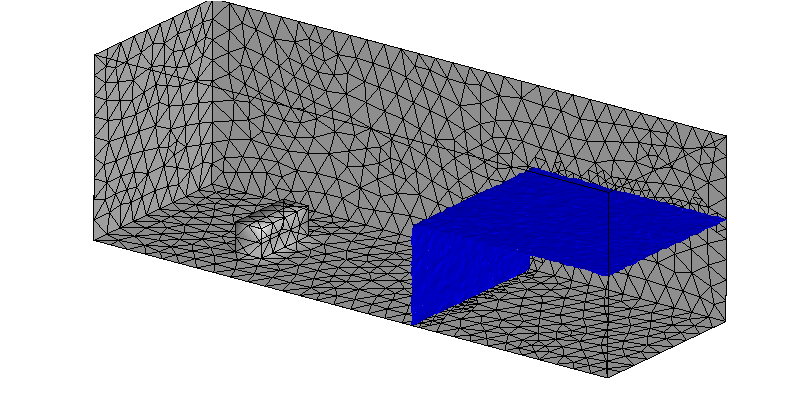
\includegraphics[width=\textwidth]{3D_Dam_t0.eps}
	%			\caption{$ t=0.0 $}
	% 		\end{subfigure}
	% 			~
	% 		\begin{subfigure}[]{0.45\textwidth}
	% 		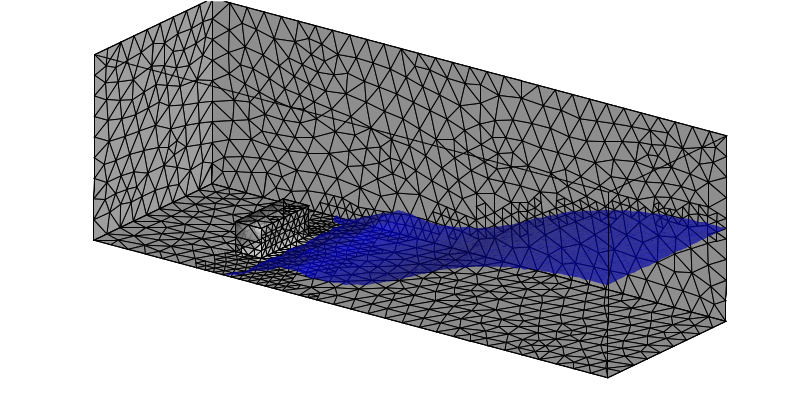
\includegraphics[width=\textwidth]{3D_Dam_t0_44.eps}
	% 		\caption{$ t=0.35 $}
	% 		\end{subfigure}
	% 		~
	% 		\begin{subfigure}[]{0.45\textwidth}
	% 		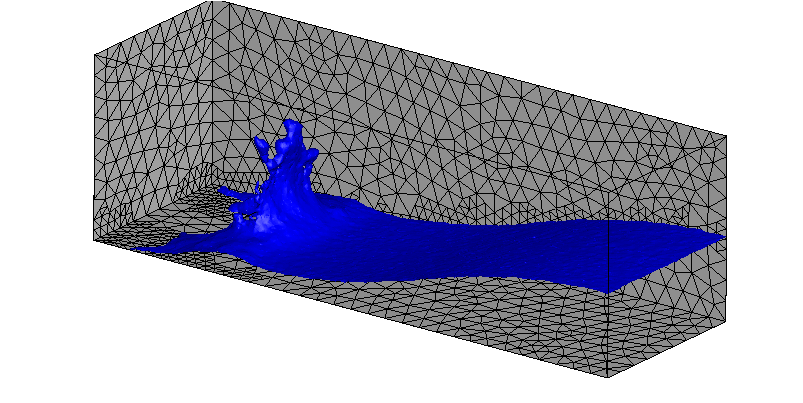
\includegraphics[width=\textwidth]{3D_Dam_t0_62.eps}
	% 		\caption{$ t=0.5 $}
	%		\end{subfigure}
	% 		 		~
	% 		\begin{subfigure}[]{0.45\textwidth}
	% 		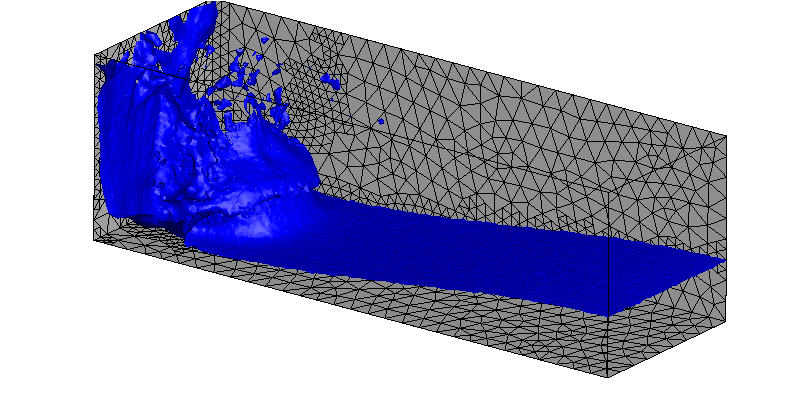
\includegraphics[width=\textwidth]{3D_Dam_t1_00.eps}
	% 	   \caption{$ t=0.8 $}
	% 	   \end{subfigure}	
	% 	   ~
	% 	   \begin{subfigure}[]{0.45\textwidth}
	% 	   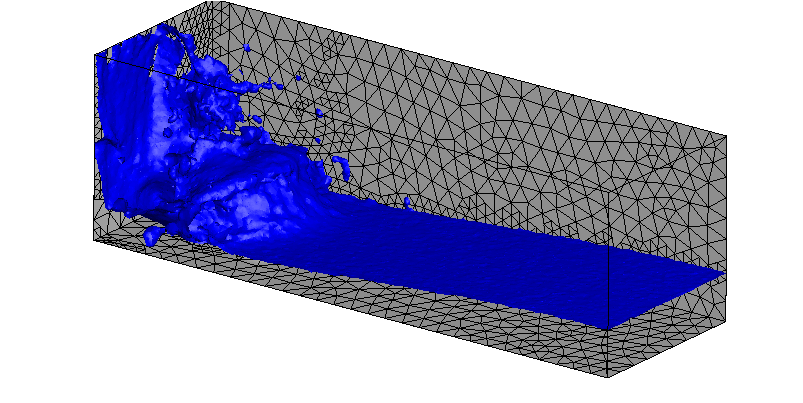
\includegraphics[width=\textwidth]{3D_Dam_t1_20.eps}
	% 	    \caption{$ t=0.5 $}
	% 	   	\end{subfigure}
	% 	    		 		~
	% 	    \begin{subfigure}[]{0.45\textwidth}
	% 	    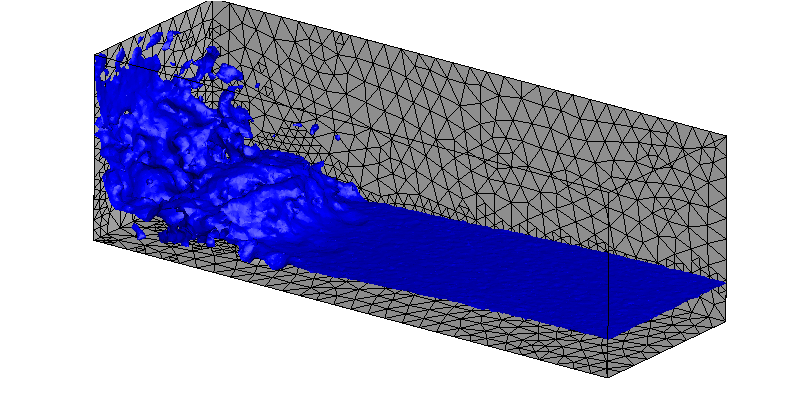
\includegraphics[width=\textwidth]{3D_Dam_t1_40.eps}
	% 	   \caption{$ t=0.8 $}
	% 	   \end{subfigure}		
	% 	\end{center}
	% 	\caption{(\textcolor{red}{TODO}: Ikişer resimden 3 sıra olabilir bu figur, detaylarin gorunmesi icin. Basılı figurde kontrast sıkıntısından oturu detaylar seçilemiyor)Snopshots of interface topolgy for 3D broken dam problem for $ N=3 $ and $ h=0.1 $. }
	% 	\label{Fig:3DDamBreakInterface}
	% \end{figure}
	
	
	%%
	\begin{figure}[ht!]
		\begin{center}
			\begin{subfigure}[]{0.3\textwidth}
				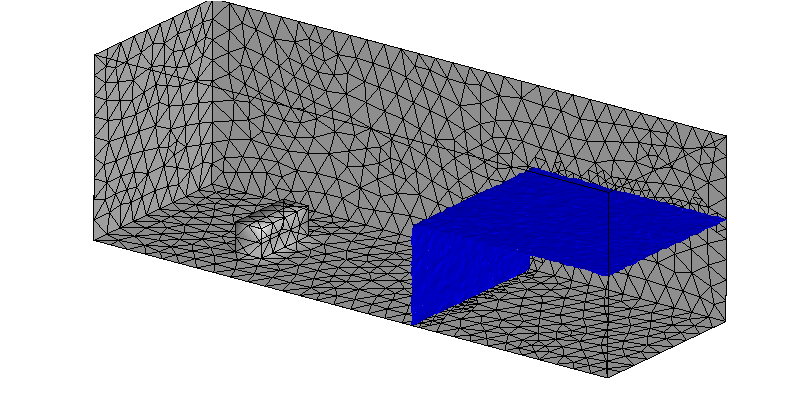
\includegraphics[width=\textwidth]{3D_Dam_t0.png}
				\caption{$ t=0.0 $}
			\end{subfigure}
			~
			\begin{subfigure}[]{0.3\textwidth}
				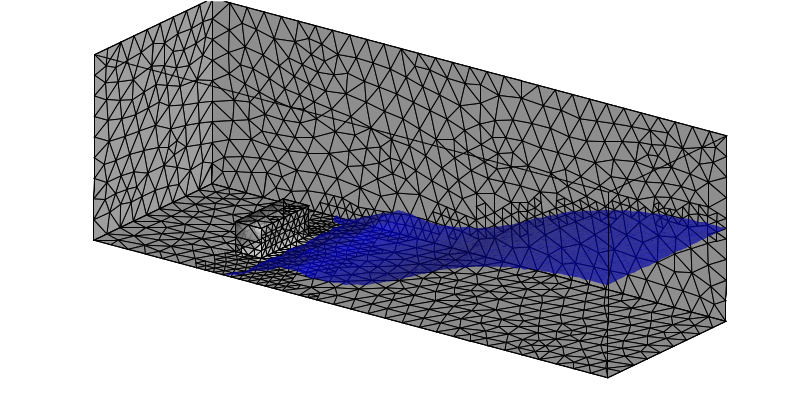
\includegraphics[width=\textwidth]{3D_Dam_t0_44.png}
				\caption{$ t=0.35 $}
			\end{subfigure}
			~
			\begin{subfigure}[]{0.3\textwidth}
				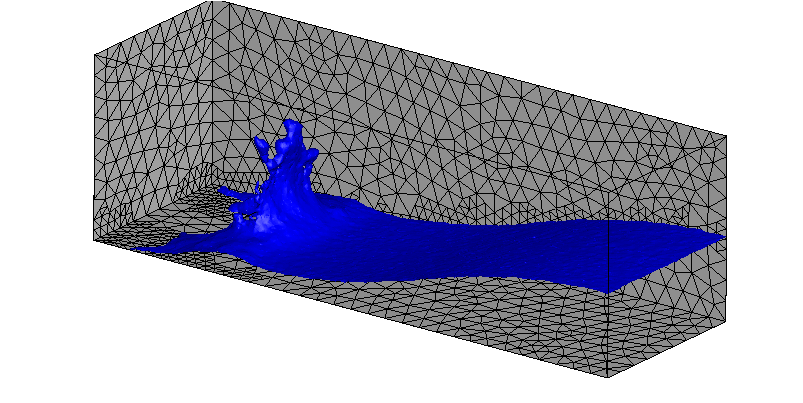
\includegraphics[width=\textwidth]{3D_Dam_t0_62.png}
				\caption{$ t=0.5 $}
			\end{subfigure}
			~
			\begin{subfigure}[]{0.3\textwidth}
				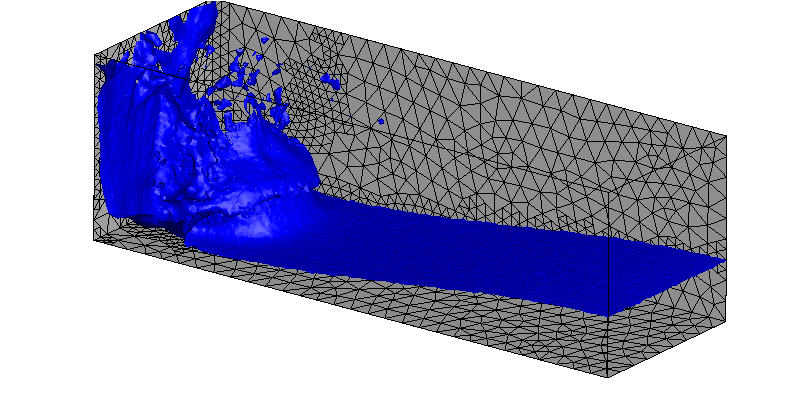
\includegraphics[width=\textwidth]{3D_Dam_t1_00.png}
				\caption{$ t=0.8 $}
			\end{subfigure}	
			~
			\begin{subfigure}[]{0.3\textwidth}
				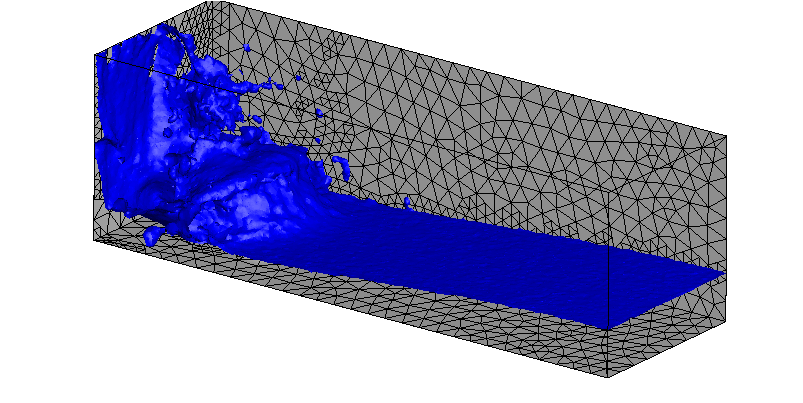
\includegraphics[width=\textwidth]{3D_Dam_t1_20.png}
				\caption{$ t=1.0 $}
			\end{subfigure}
			~
			\begin{subfigure}[]{0.3\textwidth}
				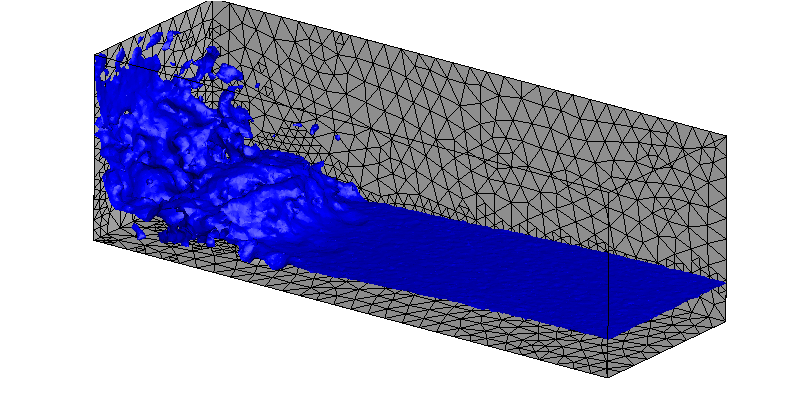
\includegraphics[width=\textwidth]{3D_Dam_t1_40.png}
				\caption{$ t=1.2 $}
			\end{subfigure}		
		\end{center}
		\caption{Snapshots of interface topolgy for 3D broken dam problem for $ N=3 $ and $ h=0.1 $. }
		\label{Fig:3DDamBreakInterface}
	\end{figure}
	
	In the experimental work of MARIN \cite{SPHERIC}, pressure histories on the rectangular obstacle are measured by eight sensors, four located on the front wall and four on the top wall. \Aref{Fig:3DDamBreakPressure} presents computed pressure history on the first and third sensor location (see \cite{SPHERIC} for details) for fixed and $ l_M = 1 $ grids. The instant that the water wave hits the obstacle is measured as $ t=0.4\;\text{s} $, which is well approximated by the current solution. Simulation and the experiment show good agreement except the magnitude of the impact pressure which is under-predicted by the numerical solution, especially with the fixed grid. This difference was also observed in other reference solutions using different techniques such as VOF \cite{kleefsman_volume--fluid_2005} and Smoothed Particle Hydrodynamics (SPH) \cite{lee_application_2010}.   
	
	%%
	\begin{figure}[ht!]
		\begin{center}
			\begin{subfigure}[]{0.45\textwidth}
				\includegraphics[width=\textwidth]{Pr3D_lm_1.eps}
				\caption{location 1}
			\end{subfigure}	
			~
			\begin{subfigure}[]{0.45\textwidth}
				\includegraphics[width=\textwidth]{Pr3D_lm_3.eps}
				\caption{location 3}
			\end{subfigure}		
			
		\end{center}
		\caption{(\textcolor{red}{TODO}: Cizgiler birbirine karismis. Birsey yapilabilir mi? Figurler biraz buyutulebilir belki. Eksen rakamlari buyutulmeli. Fixed ve adapted grid cozumleri cok benzer. Bu fixed grid'in zaten fazla iyi oldugunu gosteriyor. Keske daha coarse alinsaymis ve $ l_M = 1 $ degil 2, 3 yapilarak cozumun iyilestigi gosterilebilseymis. Yapilabilir miydi bu? Su anda adaptaion'ın kiymeti pek iyi anlatilamiyor)Comparison of computed pressure histories with experimental measurements \cite{SPHERIC}.}
		\label{Fig:3DDamBreakPressure}
	\end{figure}
	
	\textcolor{red}{TODO}: Adapted mesh icin zamanla eleman sayisindaki degisimle ilgili fikir verecek sayilar verilebilir mi? Mesela 1.2 s'ye kadar maksimum ne oluyor eleman sayisi?
	
	
	
	
	\section{Conclusion}
	A high-order, fully discontinuous Galerkin method for the solution of incompressible multiphase flows on unstructured adaptive meshes is presented. With the proposed numerical framework, the mass is well conserved even in the coarse grid solutions without introducing any special treatment or modification of the level set formulation. Velocity, pressure and interface modeling uses the same high order polynomial space preventing the interpolation of the field variables, increasing the efficiency. All implicit systems are solved with a matrix-free, $ p $-multigrid approach, reducing the memory requirement. In the adaptive method, the computation is localized mostly near the moving interfaces; reducing the computational cost significantly compared with the use of uniform mesh over the whole domain. The solution procedure given in this paper is trivially parallelizable. As a future work, parallelization of the method on all GPU-CPU platforms will be considered using recently created unified multi-threading language, OCCA \cite{medina_occa:_2014}.  
	
	%\clearpage
	%\end{linenumbers}
	
	
	
	
	\section{Acknowledments}
	A. Karakus thanks Dr. Rajesh Gandham, Dr. David Medina and Dr. Jesse Chan for their helpful discussions and valuable comments. The work of A. Karakus is partially supported by the Scientific and Technological Research Council of Turkey (TUBITAK) International Doctoral Research Fellowship Program (2214).
	%%%%%%\end{linenumbers}
	%%% ----------------------------------------------------------------
	%%
	%\bibliographystyle{abbrv}
	\bibliographystyle{unsrt}
	\bibliography{PAPER_MF} 
	
	\textcolor{red}{TODO}: referans listesi elden gecmeli. Pek cok referansin sonunda anlasilmaz sayilar var. Ilk makalemiz referans listesinde yok. 4 nolu referansta November'a gerek yok. Ikinci makalemiz basildi ve o sekilde guncellenmeli. 51 nolu referansta R ve T buyuk harf olmali. 59 referans fazla bir makale icin, 40'li sayilar daha iyi olur. Mumkunse azaltilsin.
	
\end{document}  % The End





%%%
%\begin{figure}[ht!]
%	\begin{center}
%	\begin{subfigure}[]{0.23\textwidth}
%			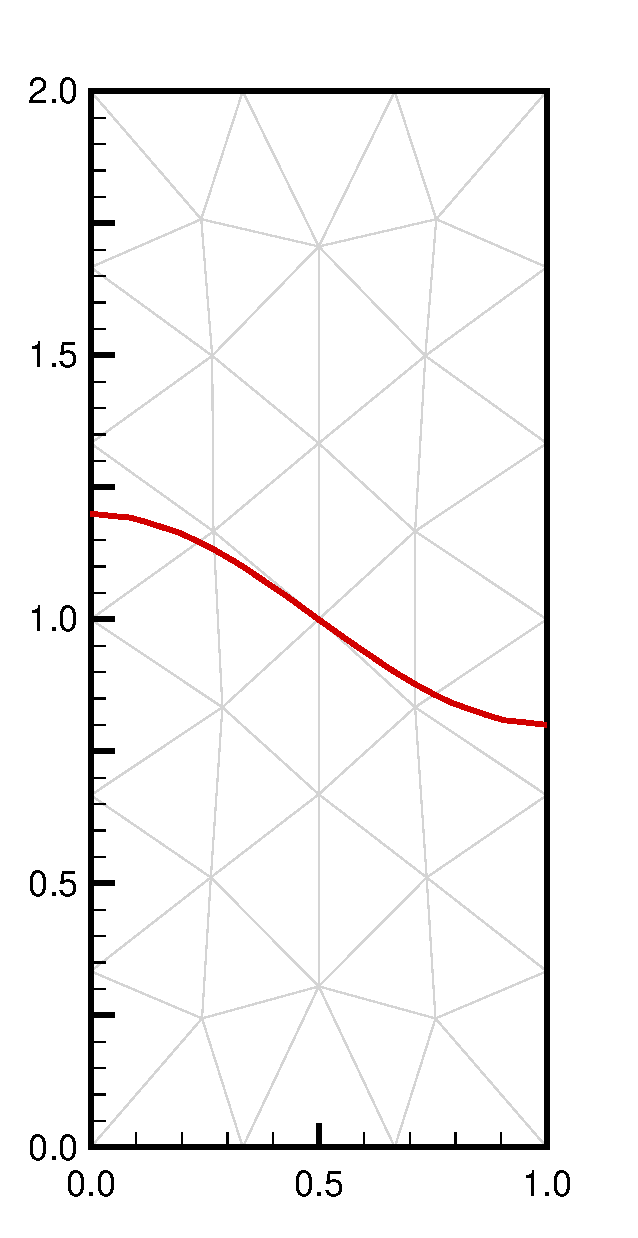
\includegraphics[width=\textwidth]{StandingWave_N3_a2_L0.eps}
%			\label{Fig:StandingWave_N3_a2_L0}
%			\caption{$ l_{M} = 0 $}
%	\end{subfigure}
%		~
%	\begin{subfigure}[]{0.23\textwidth}
%			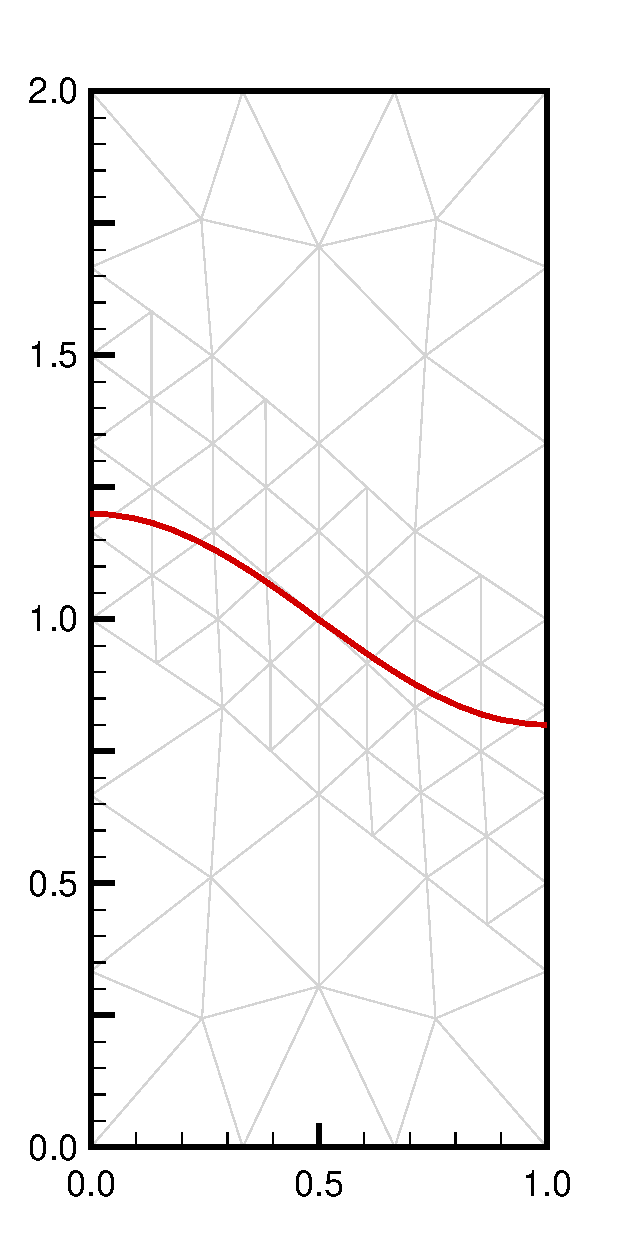
\includegraphics[width=\textwidth]{StandingWave_N3_a2_L1.eps}
%			\label{Fig:StandingWave_N3_a2_L1}
%			\caption{$ l_{M} = 1 $}
%	\end{subfigure}
%			~
%	\begin{subfigure}[]{0.23\textwidth}
%				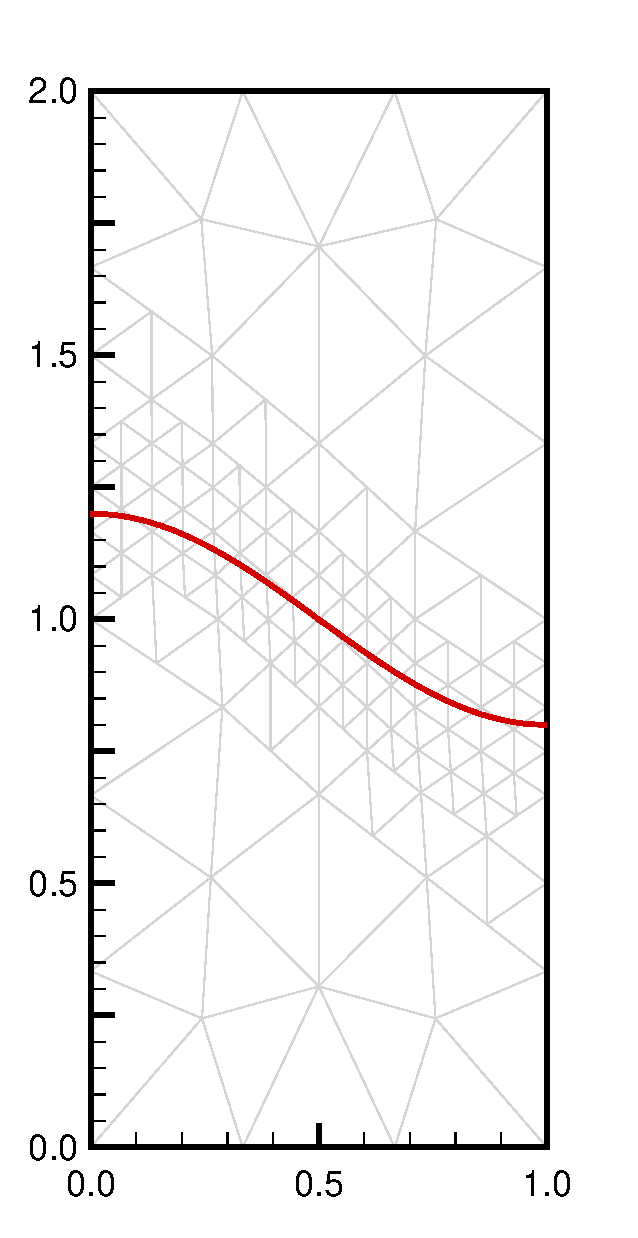
\includegraphics[width=\textwidth]{StandingWave_N3_a2_L2.eps}
%				\label{Fig:StandingWave_N3_a2_L2}
%				\caption{$ l_{M} = 2 $}
%    \end{subfigure}
%				~
%	\begin{subfigure}[]{0.23\textwidth}
%					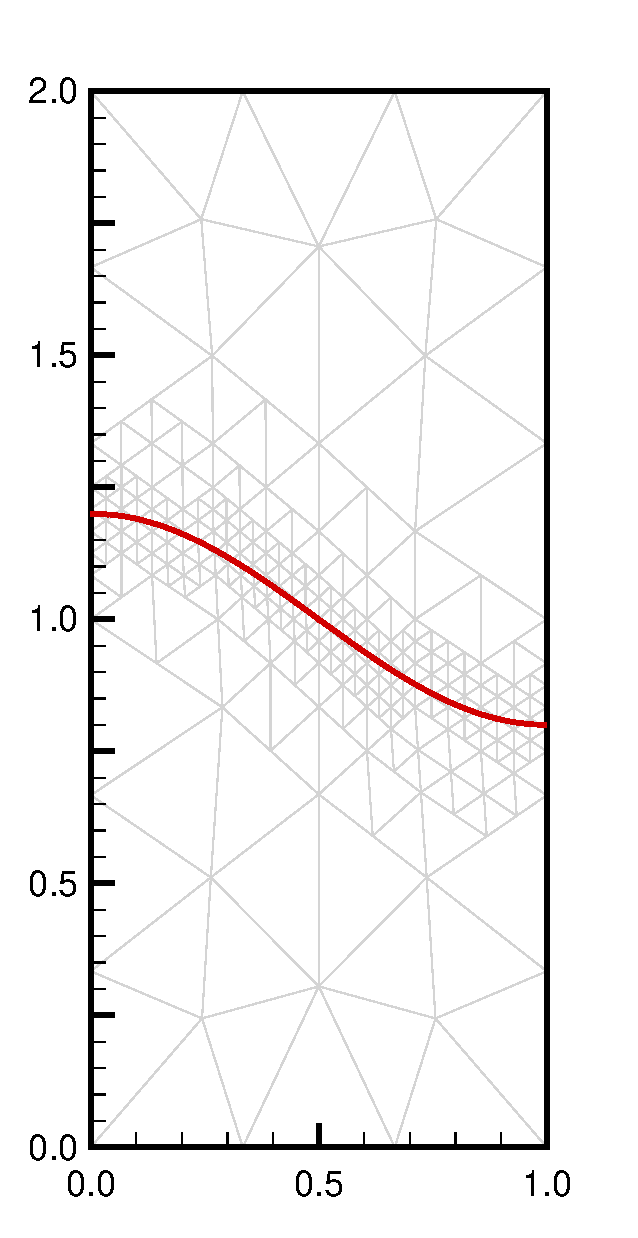
\includegraphics[width=\textwidth]{StandingWave_N3_a2_L3.eps}
%					\label{Fig:StandingWave_N3_a2_L3}
%					\caption{$ l_{M} = 3 $}
%	\end{subfigure}
%	\end{center}
%	\caption{Standing wave problem adapted grids and  interface shapes for  $ a_0 = 0.2 $ and $ N=3 $ at $ t = 0 $. }
%	\label{Fig:StandingWave_N3_a2}
%\end{figure}
